\documentclass[]{article}

\usepackage{graphicx,wrapfig}

%opening
\title{Installation instructions}
\author{lspr98}

\begin{document}

\maketitle

\begin{abstract}
	This document guides you through the process of building and installing the mod into a Profitec GO machine. These instructions are just my recommendations of installing the mod. Please read through the whole document before starting the build, to see what awaits you. 
\end{abstract}

\section{}
\subsection{Building the display unit}
\subsubsection{Printing the housing}
\begin{minipage}[t]{0.5\linewidth}
	\vspace{0pt}
	Print the two \textbf{.stl} files in the hardware folder using a filament of your choice. Orient the parts as shown in the screenshot from PrusaSlicer. Set the \textbf{layer height to 0.2mm} and \textbf{enable support everywhere}.
\end{minipage}
\hfill
\begin{minipage}[t]{0.4\linewidth}
	\vspace{0pt}
	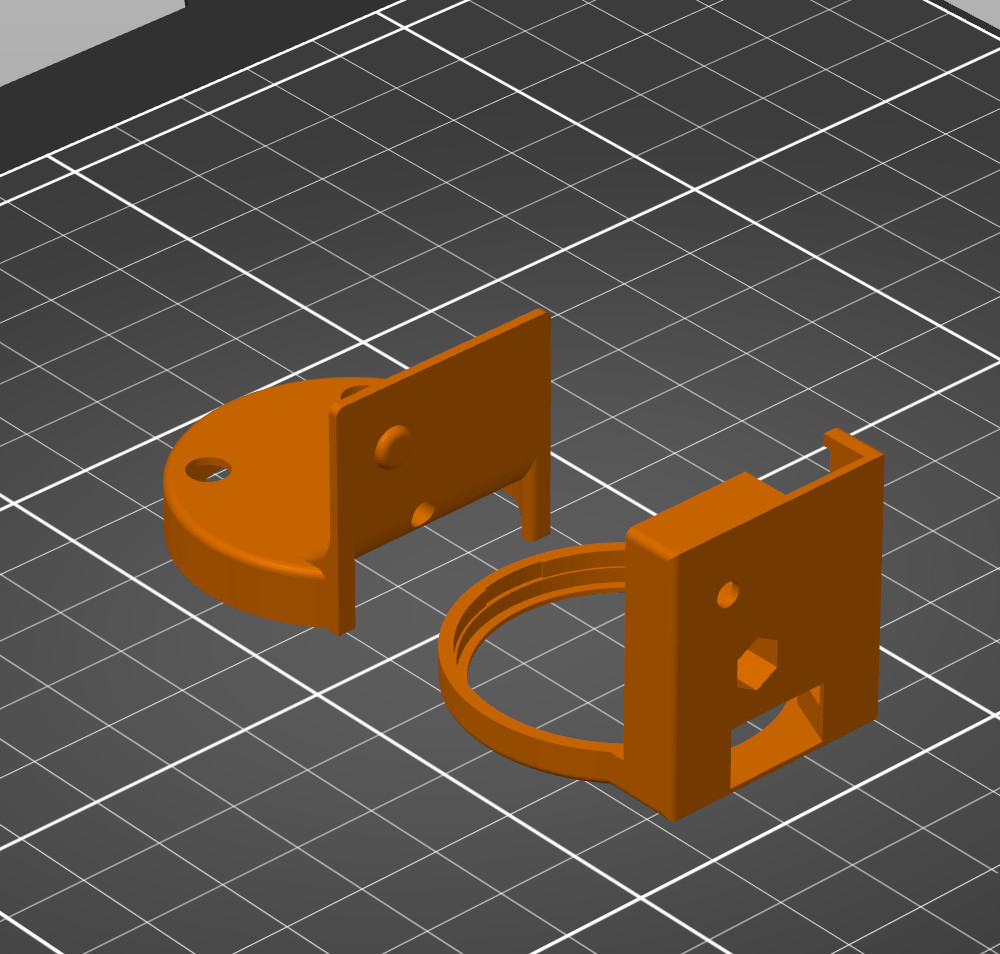
\includegraphics[width=\linewidth]{images/01_displayunit/00_print_parts.jpg}
\end{minipage}

\subsubsection{Preparing the LCD display}
\begin{minipage}[t]{0.5\linewidth}
	\vspace{0pt}
	Power up the RP2040-LCD-1.28 by plugging in a USB-C cable to confirm that it is working. It should come preloaded with a firmware that shows something on the screen. Do not peel off the screen protector yet. Take a set of tweezers and remove the two big black connectors at the back. Take something flat and sharp to gently pry the black plastic part up (there is a little notch at the short side of the connectors). After the plastic parts are removed, carefully tear off the metal connectors.
\end{minipage}
\hfill
\begin{minipage}[t]{0.4\linewidth}
	\vspace{0pt}
	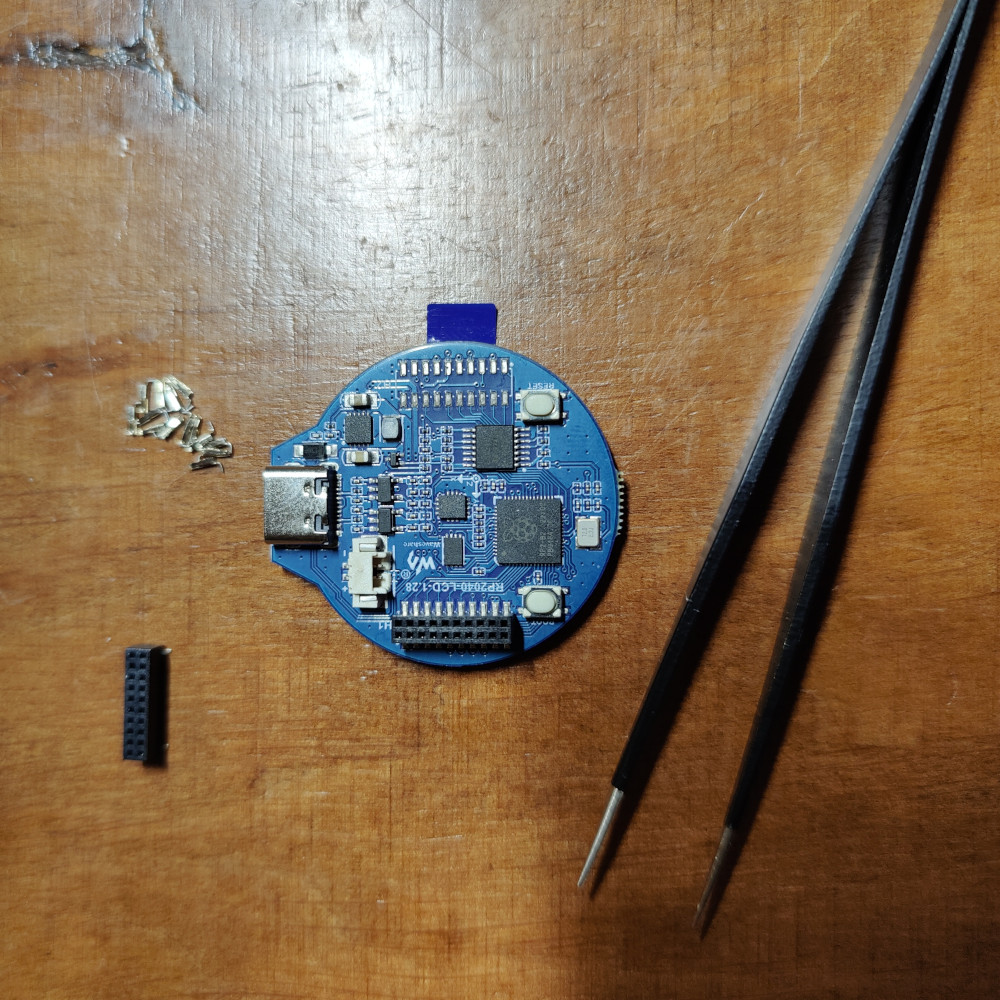
\includegraphics[width=\linewidth]{images/01_displayunit/01_remove_connectors.jpg}
\end{minipage}

\subsubsection{Preparing the display wires}
\begin{minipage}[t]{0.5\linewidth}
	\vspace{0pt}
	Cut 4 wires approximately 5cm in length. Remove the insulation of one end by around 2mm and by around 4mm at the other end for each wire. Twist all ends and apply solder.
\end{minipage}
\hfill
\begin{minipage}[t]{0.4\linewidth}
	\vspace{0pt}
	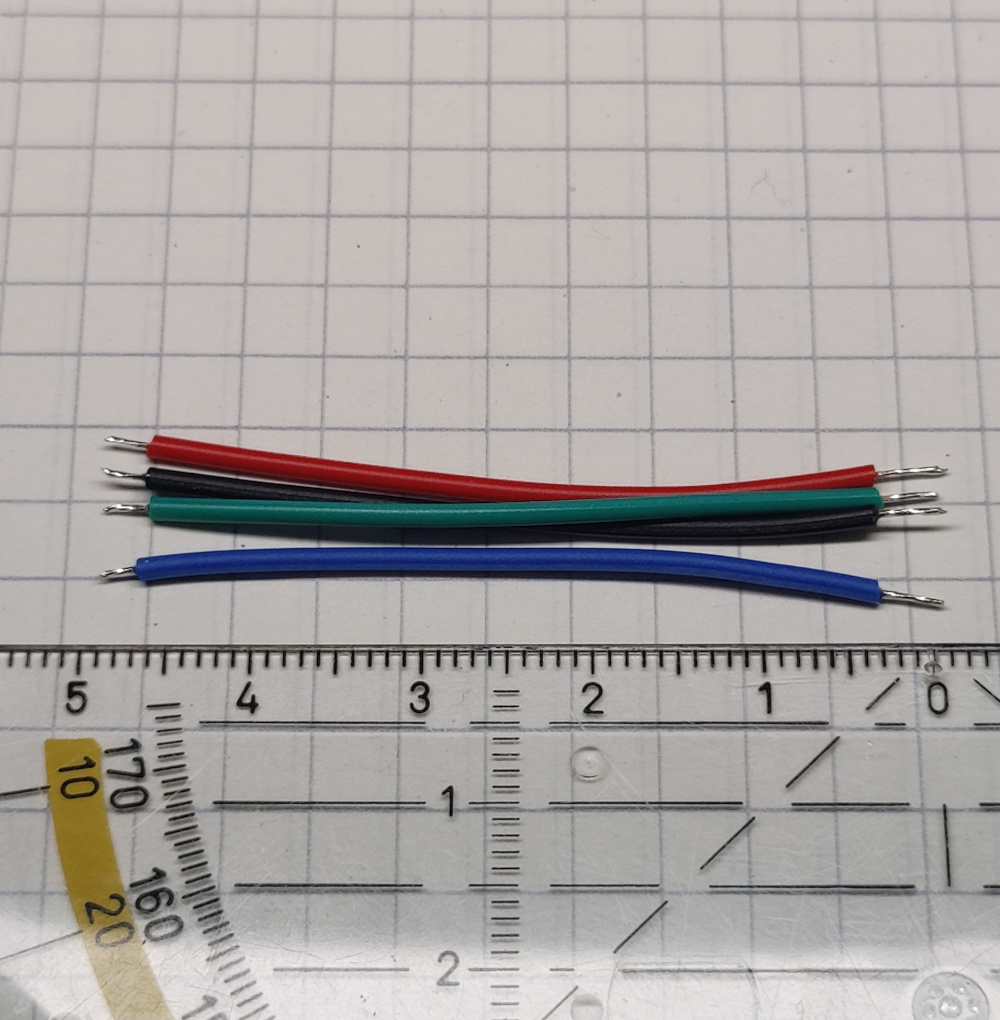
\includegraphics[width=\linewidth]{images/01_displayunit/02_wire_prepare.jpg}
\end{minipage}

\subsubsection{Tinning the required pads}
\begin{minipage}[t]{0.5\linewidth}
	\vspace{0pt}
	Apply a small amount of solder to the four pads highlighted in color. We will solder a wire to each of them in the next step. Be careful not to bridge any pads.
\end{minipage}
\hfill
\begin{minipage}[t]{0.4\linewidth}
	\vspace{0pt}
	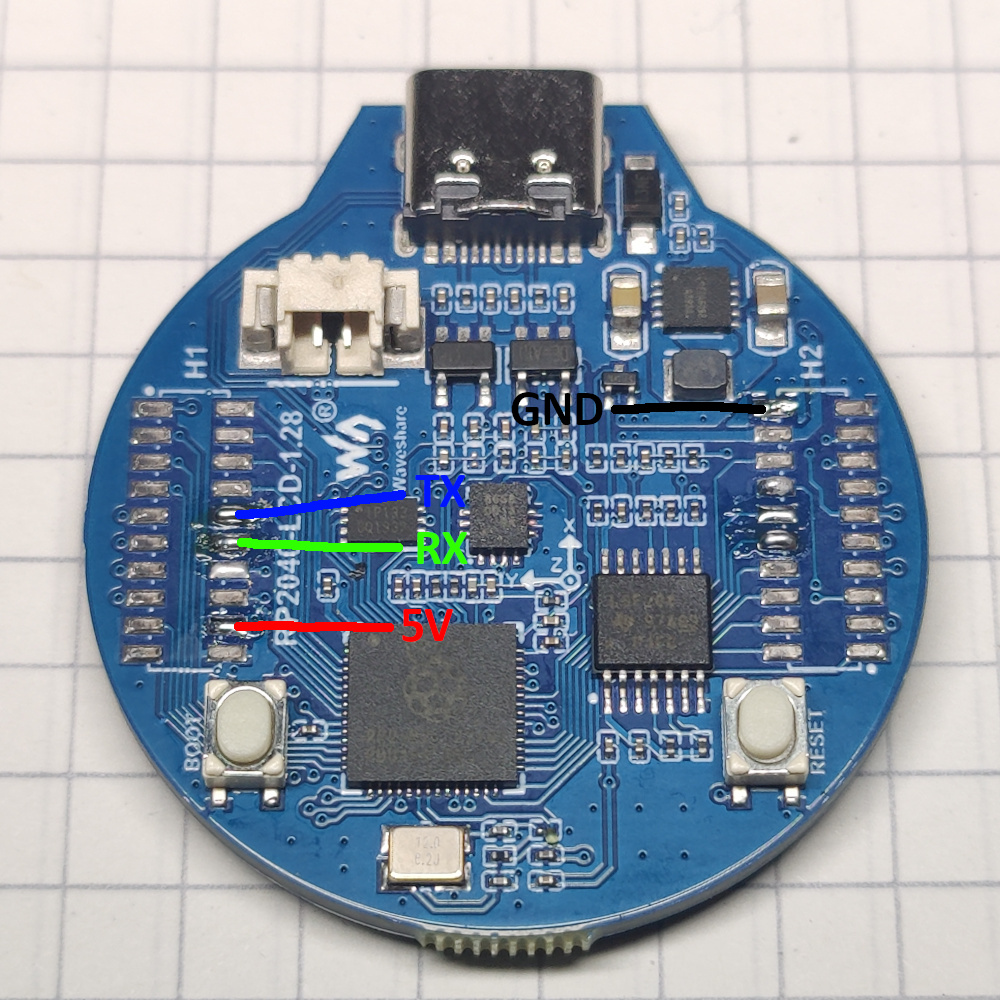
\includegraphics[width=\linewidth]{images/01_displayunit/03_tin_display.jpg}
\end{minipage}

\subsubsection{Soldering the wires to the display}
\begin{minipage}[t]{0.5\linewidth}
	\vspace{0pt}
	Solder the wires to the pads marked in the previous step.
\end{minipage}
\hfill
\begin{minipage}[t]{0.4\linewidth}
	\vspace{0pt}
	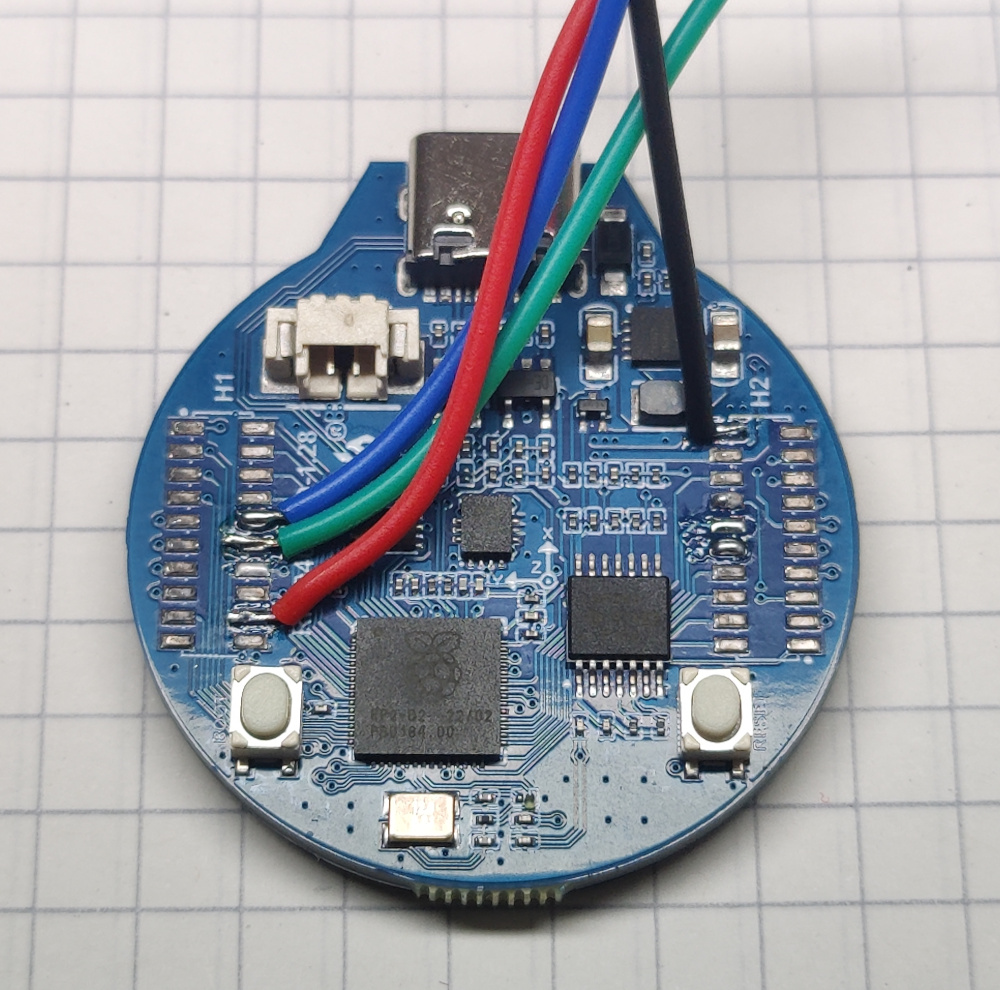
\includegraphics[width=\linewidth]{images/01_displayunit/04_solder_wires_to_display.jpg}
\end{minipage}

\subsubsection{Soldering the display plug}
\begin{minipage}[t]{0.5\linewidth}
	\vspace{0pt}
	Solder the other end of the wires to a JST-XH 4-Pin female connector. Make sure to put shrink tubing over the wires before attaching the connector. Make sure the wires are attached in the correct order to the connector (compare image).
\end{minipage}
\hfill
\begin{minipage}[t]{0.4\linewidth}
	\vspace{0pt}
	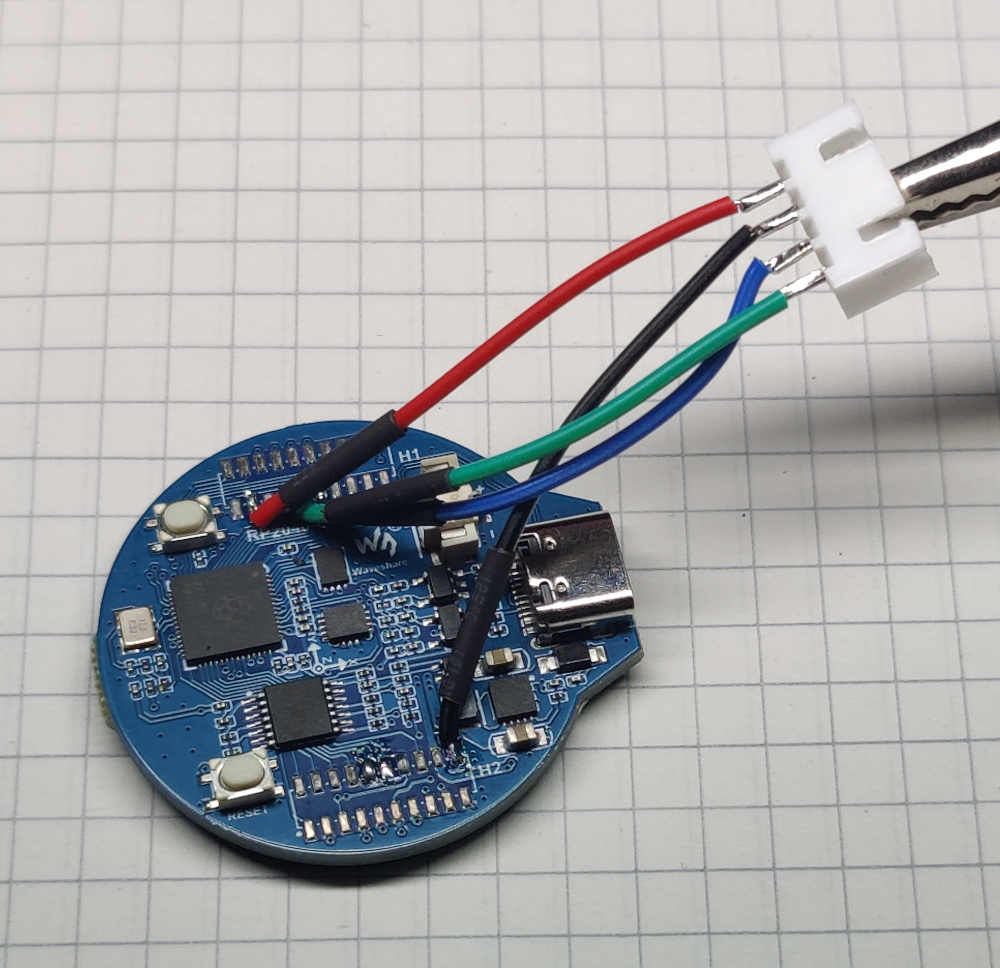
\includegraphics[width=\linewidth]{images/01_displayunit/05_solder_wires_to_plug.jpg}
\end{minipage}

\subsubsection{Applying the shrink tubing}
\begin{minipage}[t]{0.5\linewidth}
	\vspace{0pt}
	Push the shrink tubing over the uncovered wire ends and heat them up using a lighter. Do not heat up the connector too much, otherwise the pins may become lose as the plastic softens!
\end{minipage}
\hfill
\begin{minipage}[t]{0.4\linewidth}
	\vspace{0pt}
	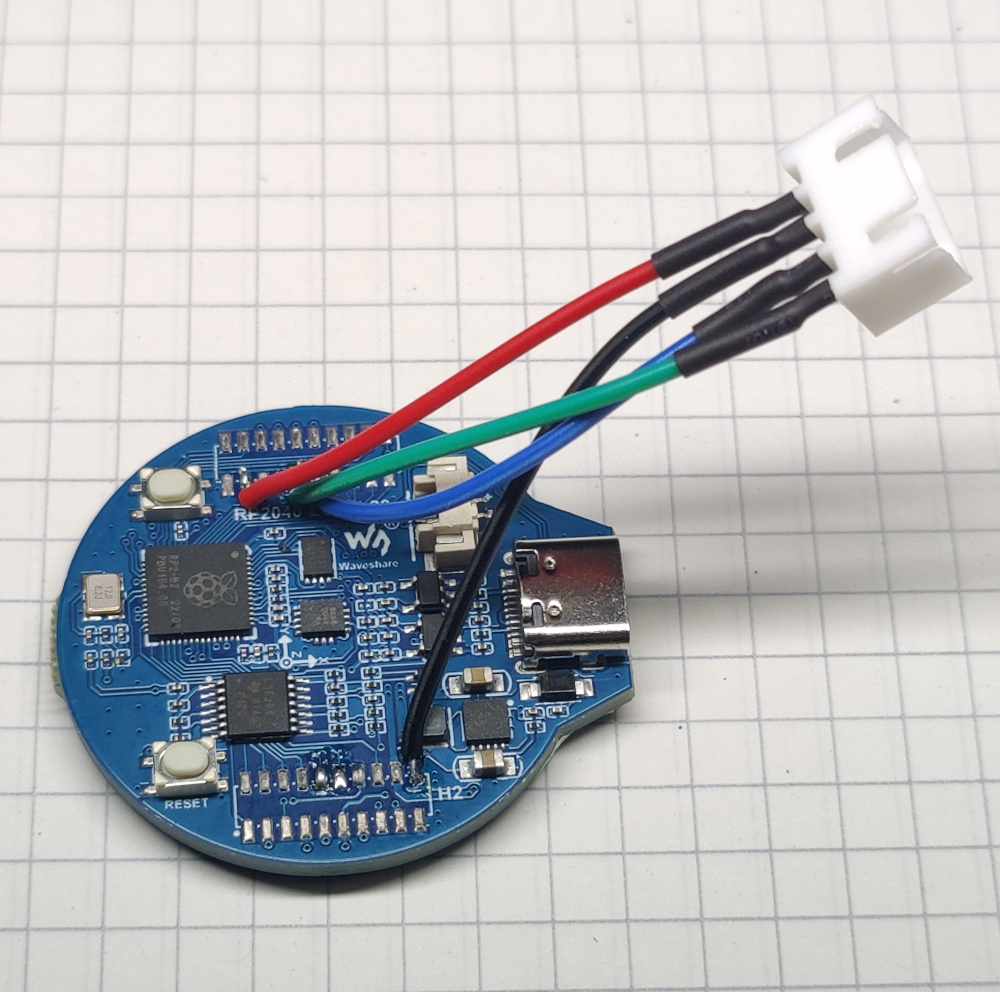
\includegraphics[width=\linewidth]{images/01_displayunit/06_shrinktubing_plug.jpg}
\end{minipage}

\subsubsection{Inserting the nut}
\begin{minipage}[t]{0.5\linewidth}
	\vspace{0pt}
	Take the M3 screw, the M3 nut and the 3d-printed Frame.stl part. Push the M3 screw through the hole that has a nut compartment at the other side. If the screw doesn't go through easily, take a screwdriver and screw it in completely. Screw on the nut onto the screw from the other side until it aligns with the surface of the 3D-printed part.
\end{minipage}
\hfill
\begin{minipage}[t]{0.4\linewidth}
	\vspace{0pt}
	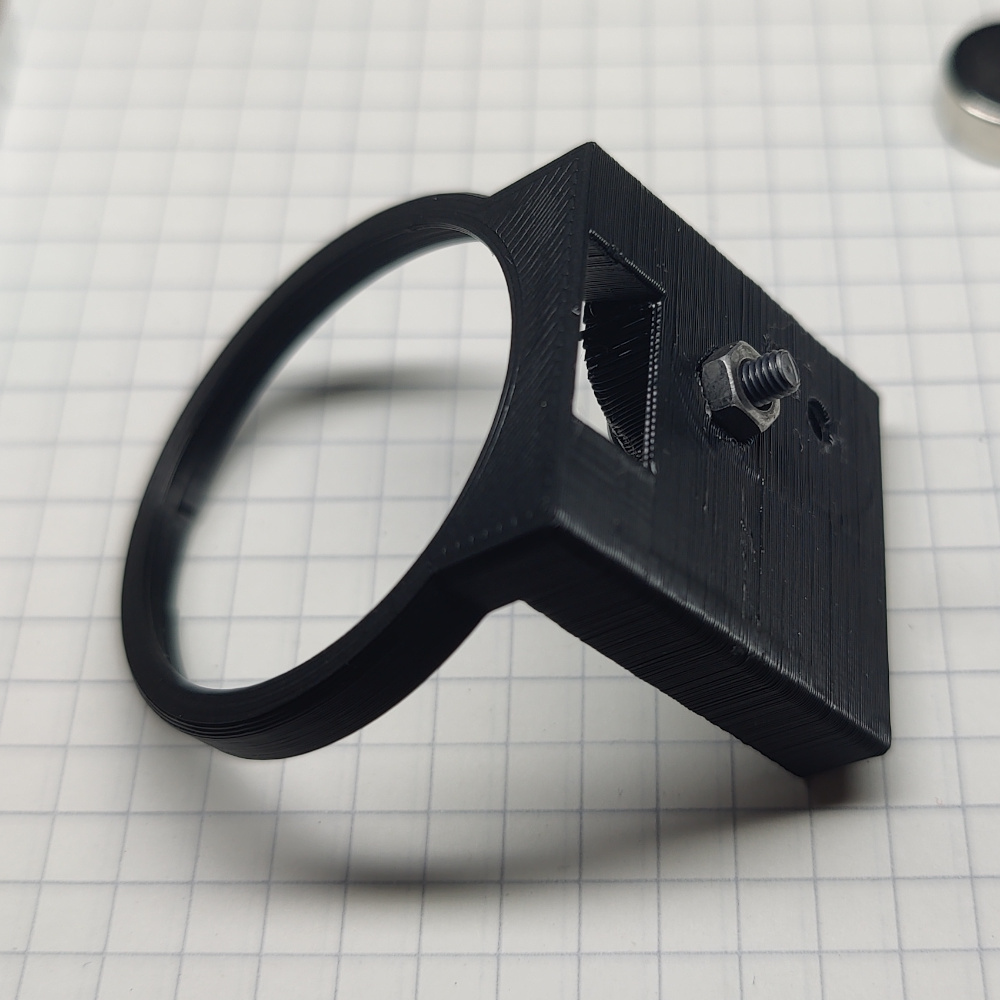
\includegraphics[width=\linewidth]{images/01_displayunit/08_prepare_nutslot.jpg}
\end{minipage}

\subsubsection{Pulling the nut in}
\begin{minipage}[t]{0.5\linewidth}
	\vspace{0pt}
	Keep screwing the M3-screw to pull the nut into the compartment until it is fully inserted (you can feel a sudden resistance when screwing). Do not apply too much force to avoid breaking the part. Remove the screw afterwards.
\end{minipage}
\hfill
\begin{minipage}[t]{0.4\linewidth}
	\vspace{0pt}
	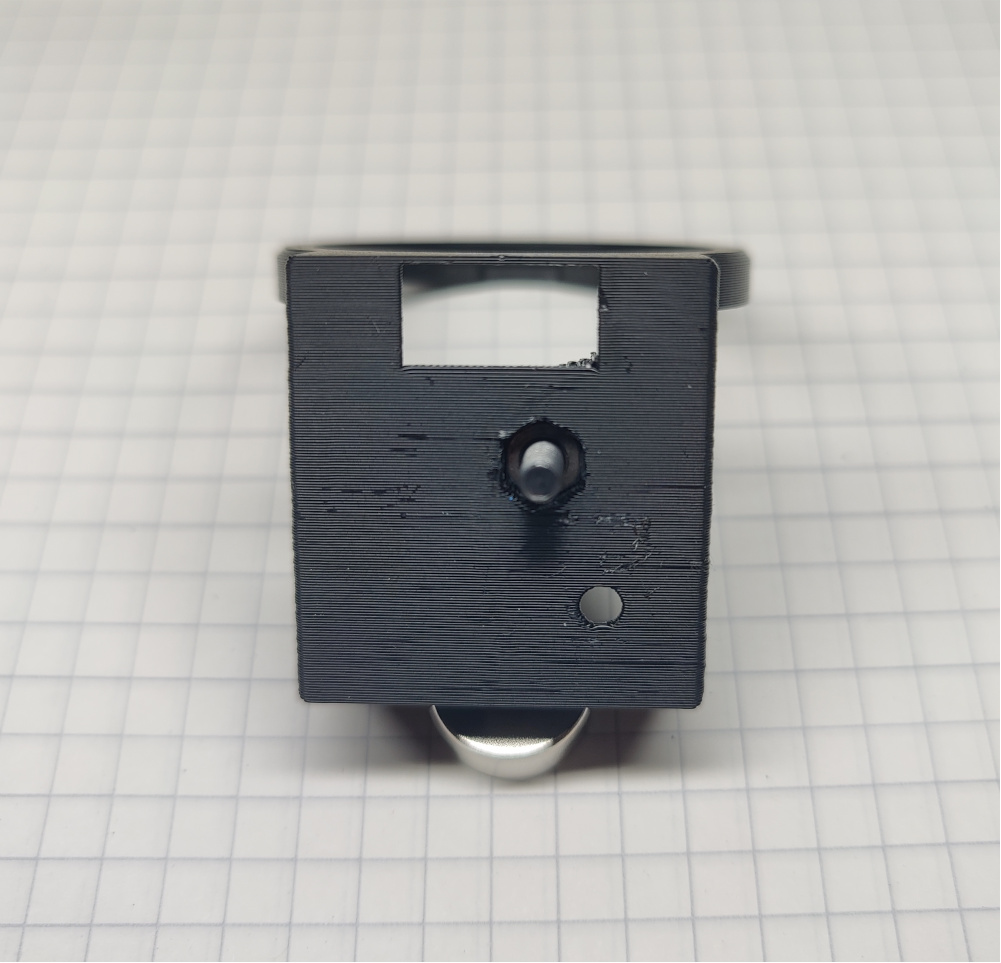
\includegraphics[width=\linewidth]{images/01_displayunit/09_pull_nut.jpg}
\end{minipage}

\subsubsection{Inserting the magnet}
\begin{minipage}[t]{0.5\linewidth}
	\vspace{0pt}
	Insert the magnet. If you use a smaller one, make sure you fix the magnet in place with glue or something. It should not be able to move afterwards. Make sure the magnet is fully inserted.
\end{minipage}
\hfill
\begin{minipage}[t]{0.4\linewidth}
	\vspace{0pt}
	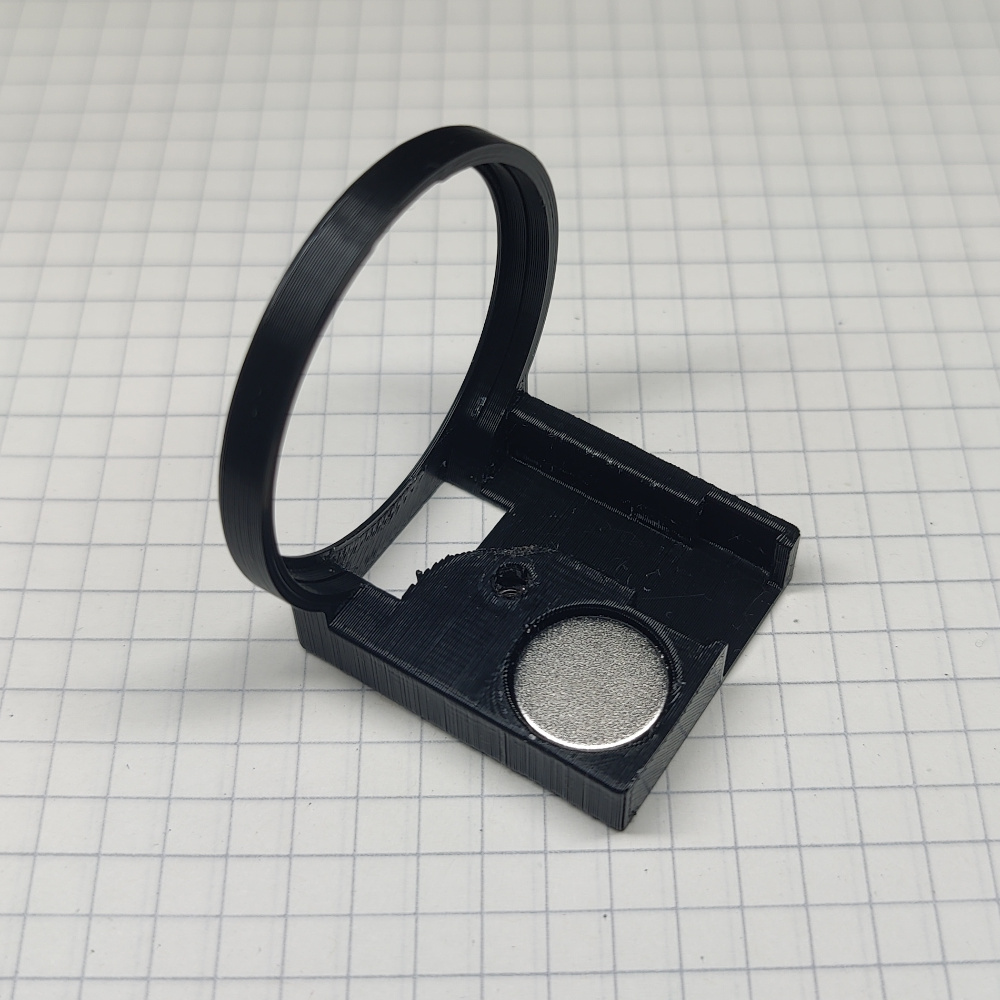
\includegraphics[width=\linewidth]{images/01_displayunit/11_insert_magnet.jpg}
\end{minipage}

\subsubsection{Aligning the display}
\begin{minipage}[t]{0.5\linewidth}
	\vspace{0pt}
	Carefully insert the display into the frame at an angle like shown in the picture. Then push it completely into the frame. It should snap in place without much force.
\end{minipage}
\hfill
\begin{minipage}[t]{0.4\linewidth}
	\vspace{0pt}
	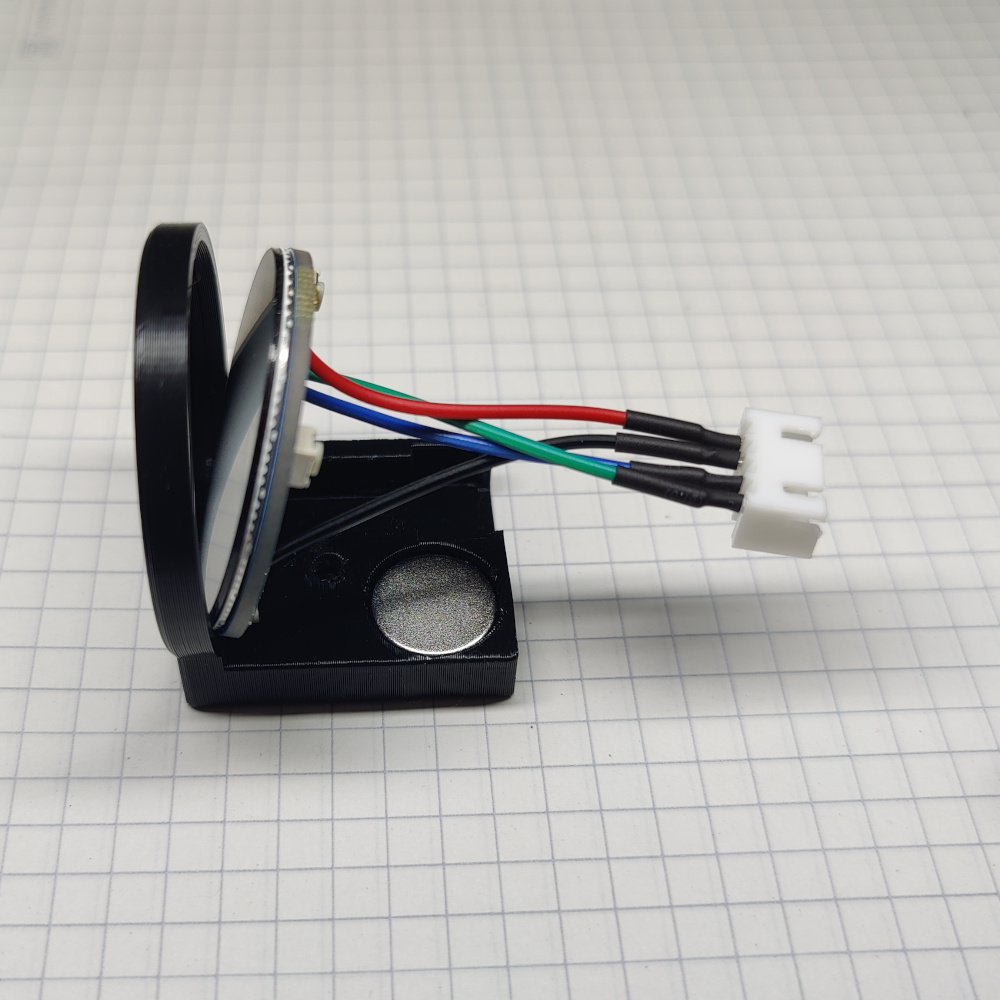
\includegraphics[width=\linewidth]{images/01_displayunit/13_insert_display.jpg}
\end{minipage}

\subsubsection{Checking display alignment}
\begin{minipage}[t]{0.5\linewidth}
	\vspace{0pt}
	If the display is inserted correctly, the PCB surface should align with the surface of the 3d-printed part. If you are having trouble to align it, check the 3D-printed part for any remaining support structures that were not removed.
\end{minipage}
\hfill
\begin{minipage}[t]{0.4\linewidth}
	\vspace{0pt}
	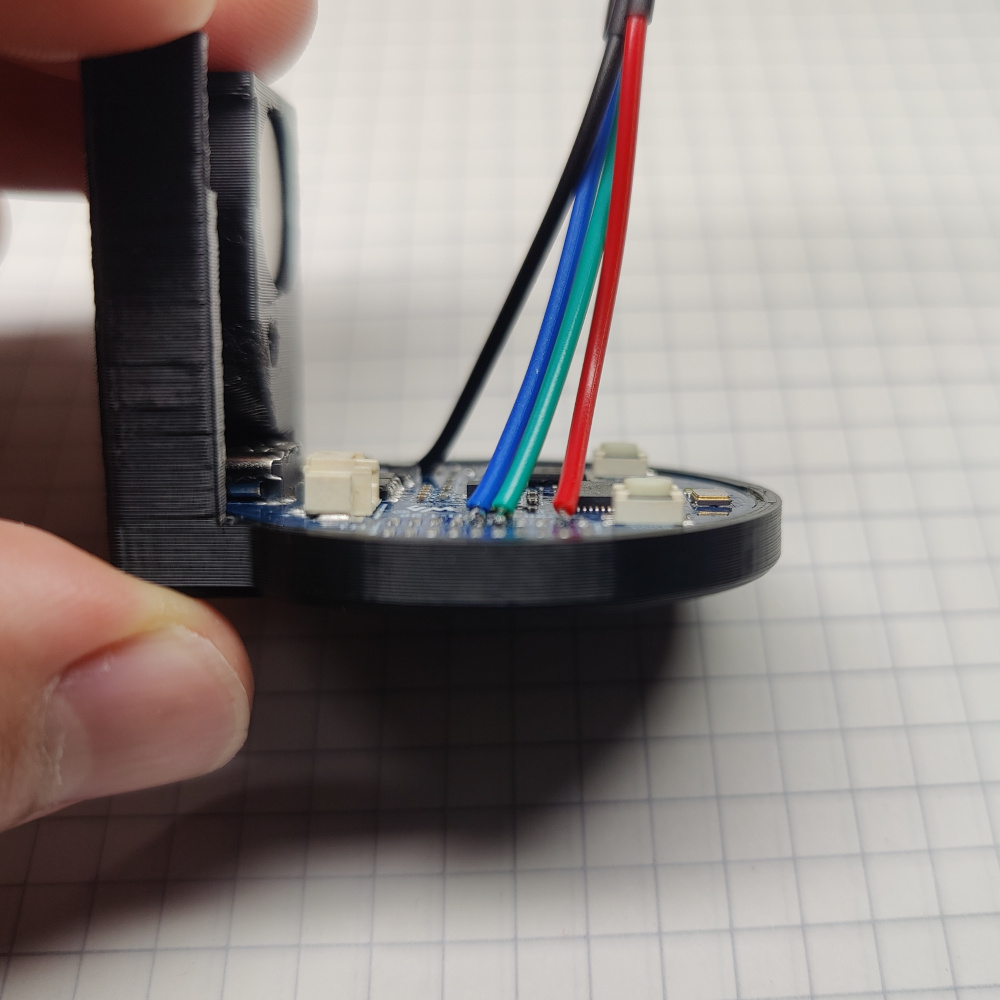
\includegraphics[width=\linewidth]{images/01_displayunit/14_check_display1.jpg}
\end{minipage}

\subsubsection{Checking USB-port alignment}
\begin{minipage}[t]{0.5\linewidth}
	\vspace{0pt}
	Verify that the USB-port at the bottom is fully accessible and not covered by the 3D-printed part.
\end{minipage}
\hfill
\begin{minipage}[t]{0.4\linewidth}
	\vspace{0pt}
	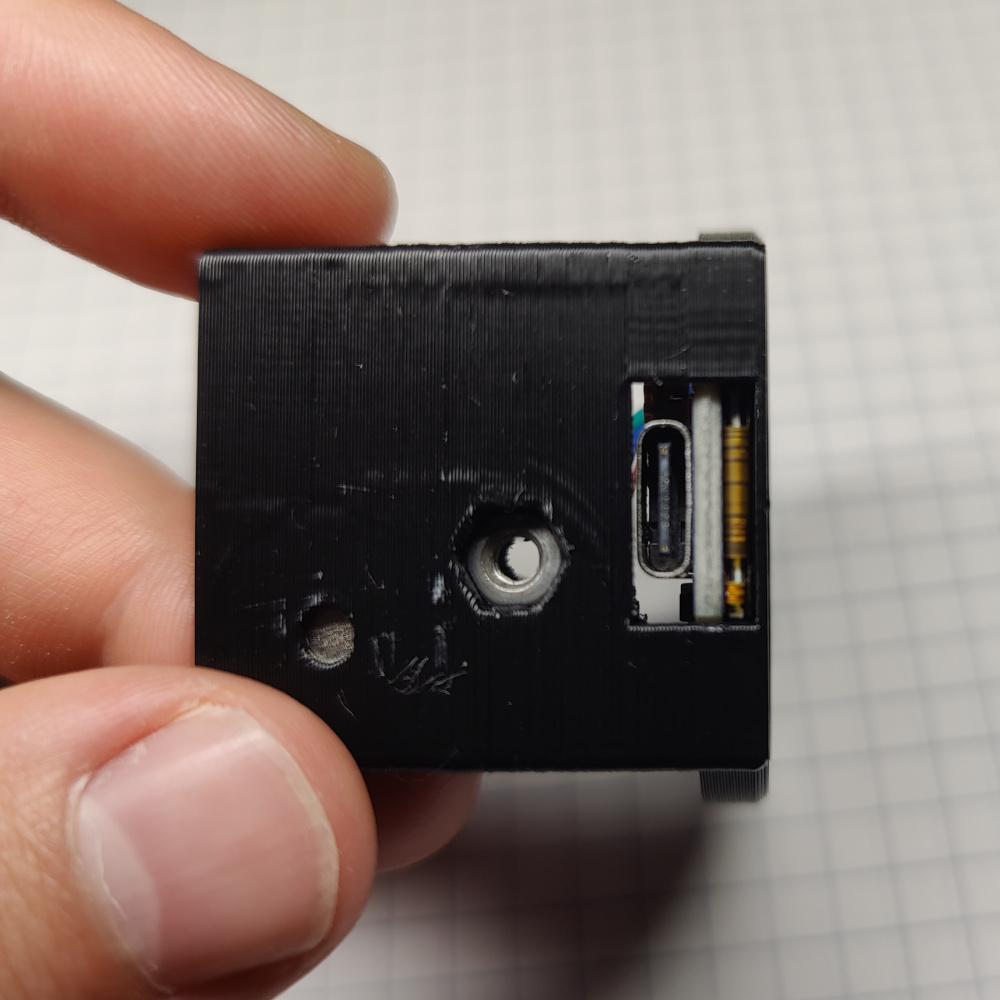
\includegraphics[width=\linewidth]{images/01_displayunit/15_check_usb.jpg}
\end{minipage}

\subsubsection{Inserting the display plug}
\begin{minipage}[t]{0.5\linewidth}
	\vspace{0pt}
	Push the JST-XH 4-Pin female connector into it's slot.
\end{minipage}
\hfill
\begin{minipage}[t]{0.4\linewidth}
	\vspace{0pt}
	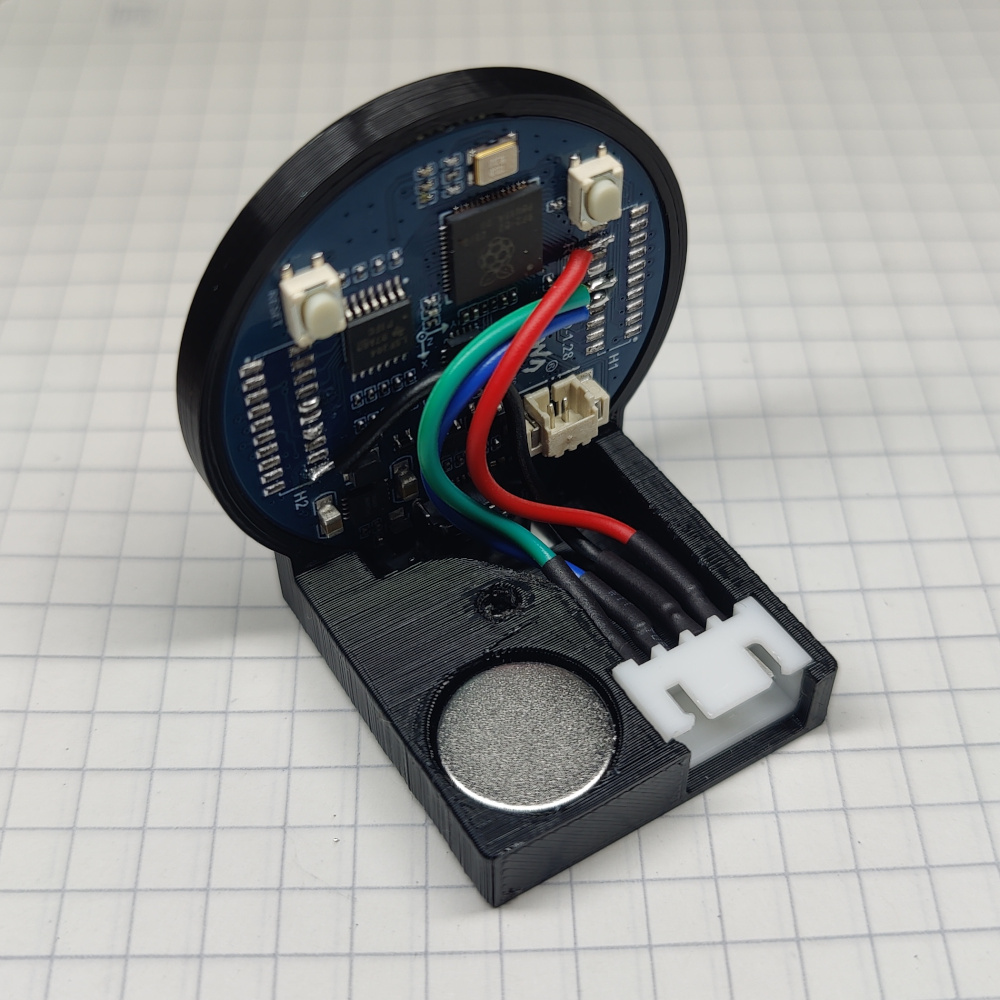
\includegraphics[width=\linewidth]{images/01_displayunit/16_insert_plug.jpg}
\end{minipage}

\subsubsection{Closing the frame}
\begin{minipage}[t]{0.5\linewidth}
	\vspace{0pt}
	Take the other 3D-printed part and close the frame by screwing the M3-screw in like shown in the picture. Be careful not to pinch any wires while doing so.
\end{minipage}
\hfill
\begin{minipage}[t]{0.4\linewidth}
	\vspace{0pt}
	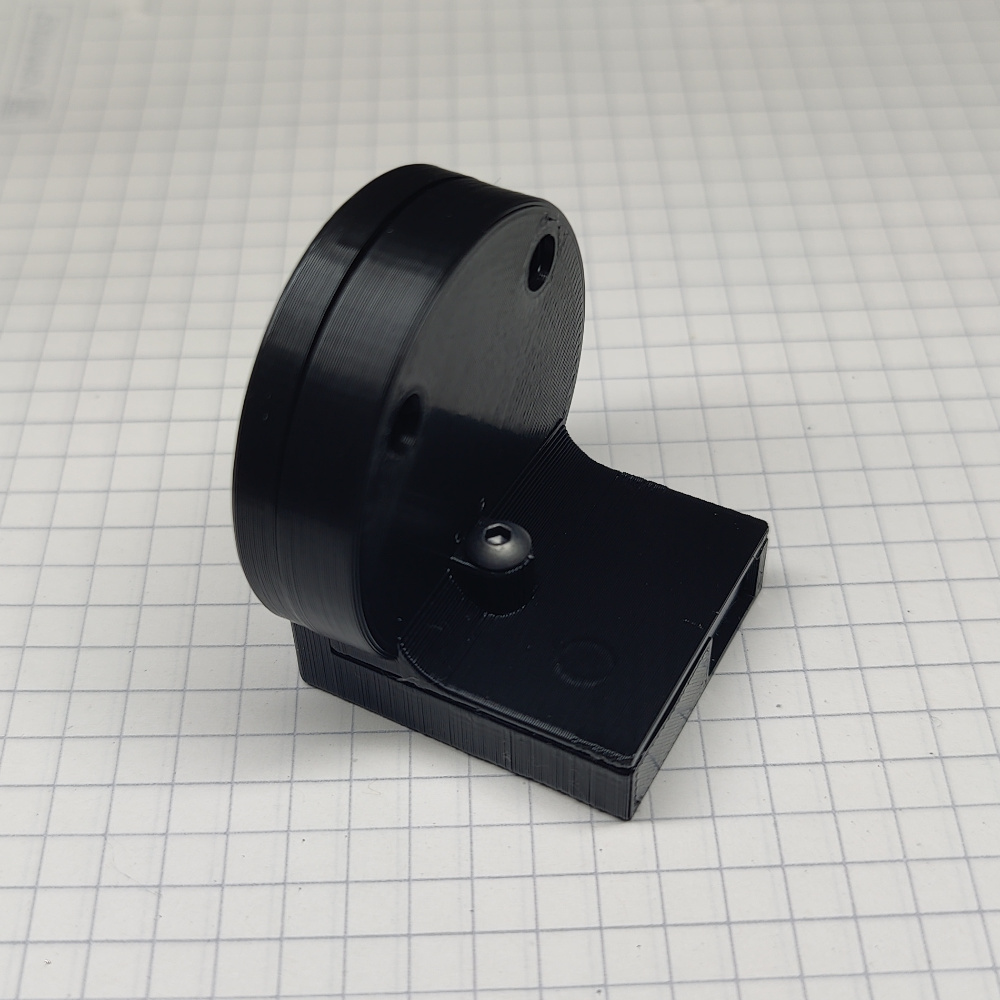
\includegraphics[width=\linewidth]{images/01_displayunit/17_close_frame.jpg}
\end{minipage}

\subsubsection{Checking the gaps}
\begin{minipage}[t]{0.5\linewidth}
	\vspace{0pt}
	If everything was done correctly, the two pieces should align, leaving (almost) no gap.
\end{minipage}
\hfill
\begin{minipage}[t]{0.4\linewidth}
	\vspace{0pt}
	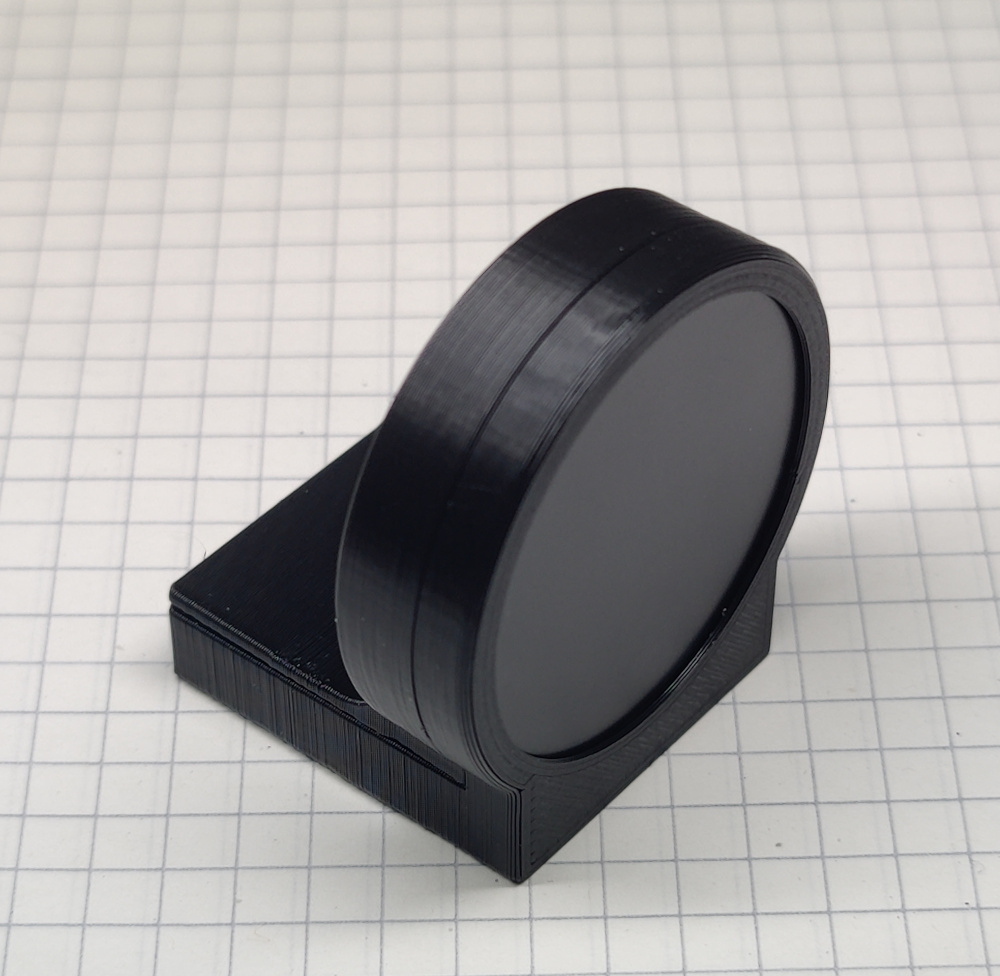
\includegraphics[width=\linewidth]{images/01_displayunit/18_check_gaps.jpg}
\end{minipage}

\subsubsection{Checking the buttons}
\begin{minipage}[t]{0.5\linewidth}
	\vspace{0pt}
	Verify that the two buttons at the back of the display are not covered or pushed by any wires and that no pins of the connector are bent.
\end{minipage}
\hfill
\begin{minipage}[t]{0.4\linewidth}
	\vspace{0pt}
	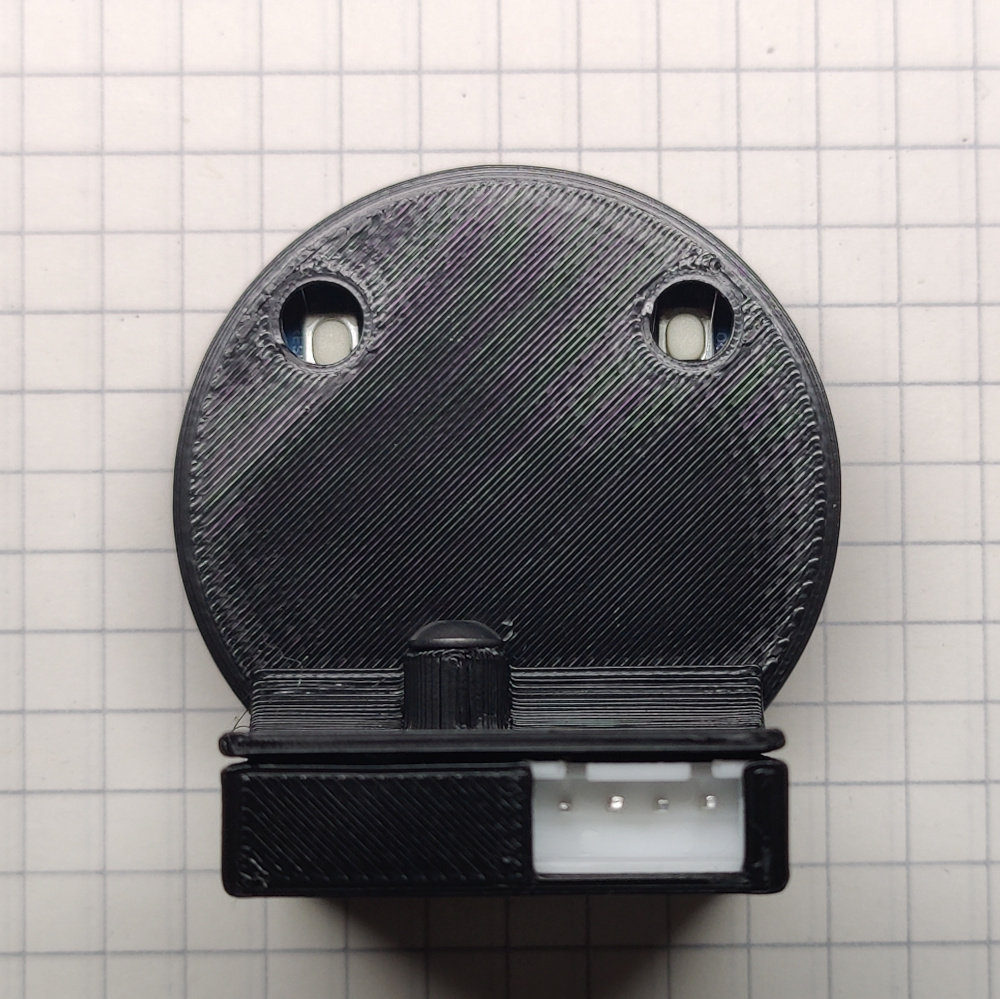
\includegraphics[width=\linewidth]{images/01_displayunit/19_check_buttons_pins.jpg}
\end{minipage}

\subsubsection{Checking the bottom}
\begin{minipage}[t]{0.5\linewidth}
	\vspace{0pt}
	Make sure no metal parts are sticking out from the bottom! The USB-port, the nut and the screw should be recessed to avoid scratching the surface of your machine.
\end{minipage}
\hfill
\begin{minipage}[t]{0.4\linewidth}
	\vspace{0pt}
	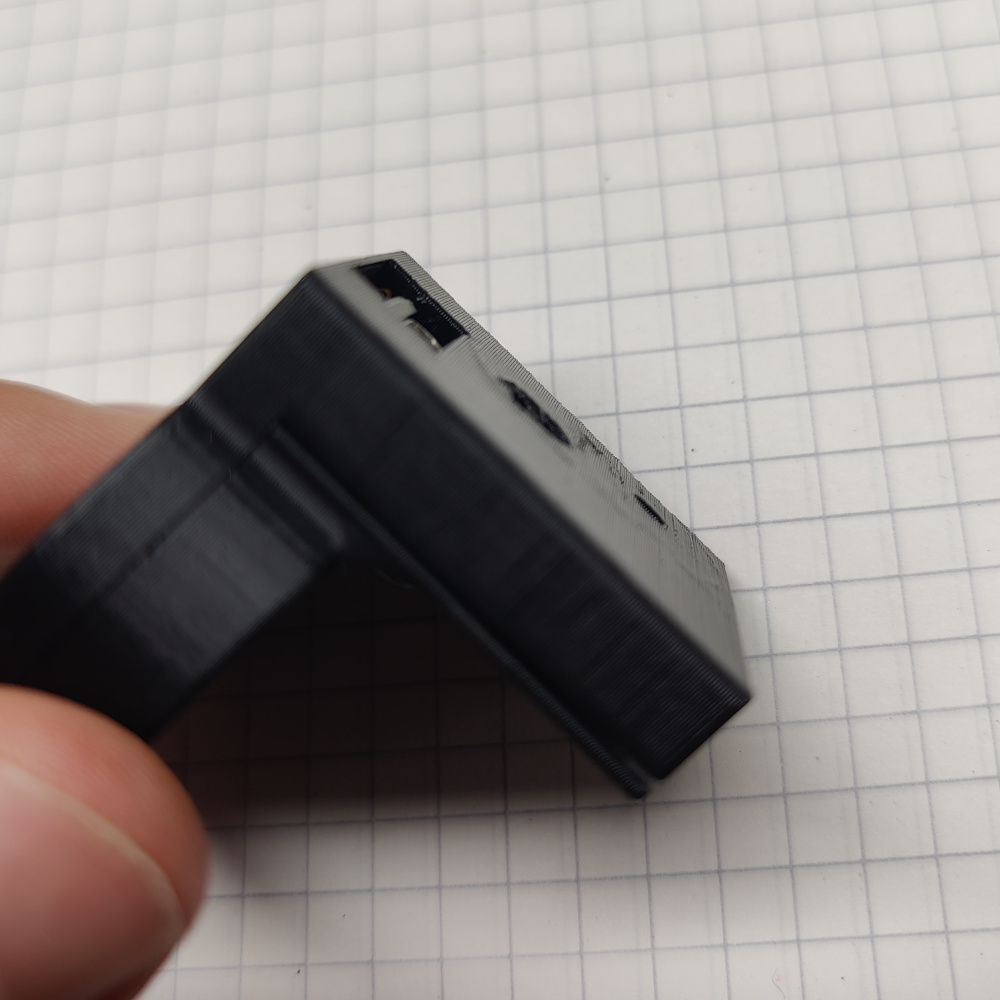
\includegraphics[width=\linewidth]{images/01_displayunit/20_check_bottom.jpg}
\end{minipage}

\subsubsection{Flashing the firmware}
\begin{minipage}[t]{0.5\linewidth}
	\vspace{0pt}
	If not done already, install VisualStudio Code and install the PlatformIO plugin for it. Clone the Github repository to your PC and open it as a PlatformIO project. Connect the display unit to your PC via a USB cable. Build and flash the firmware by pressing the highlighted button at the bottom left of the window.
\end{minipage}
\hfill
\begin{minipage}[t]{0.4\linewidth}
	\vspace{0pt}
	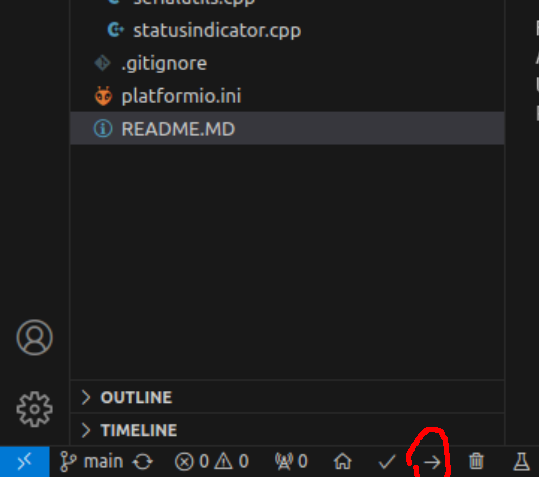
\includegraphics[width=\linewidth]{images/01_displayunit/22_build_and_upload.png}
\end{minipage}

\subsubsection{Testing}
\begin{minipage}[t]{0.5\linewidth}
	\vspace{0pt}
	If the flashing process was successful, it should show an orange ring with a question mark indicating a missing fill-level sensor. Try shaking the device for more than 2 seconds to test the shot timer.
\end{minipage}
\hfill
\begin{minipage}[t]{0.4\linewidth}
	\vspace{0pt}
	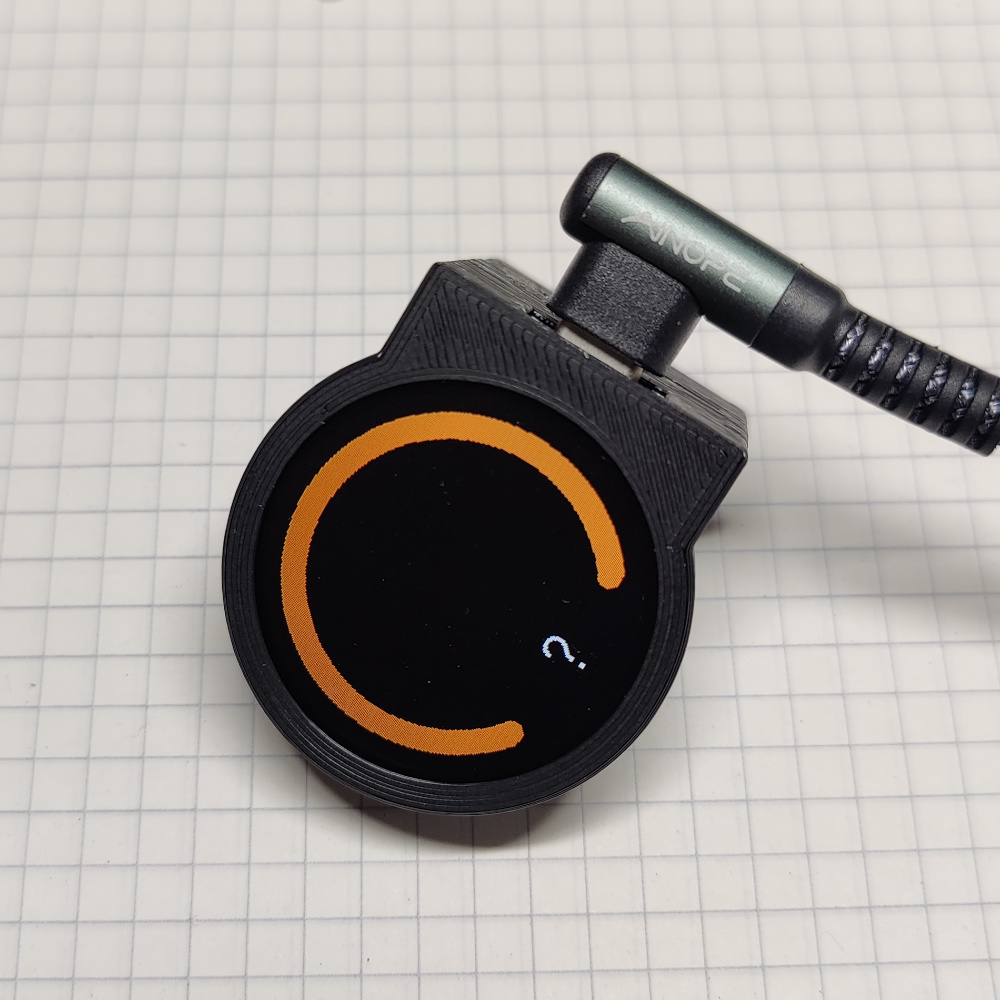
\includegraphics[width=\linewidth]{images/01_displayunit/21_check_display.jpg}
\end{minipage}


\subsection{Wire harness, level sensor and power supply}
\subsubsection{Display cable}
\begin{minipage}[t]{0.5\linewidth}
	\vspace{0pt}
	Take the old USB cable / your 4-core wire and cut it to around 40cm length. Strip the 4 wires in the cable and crimp a JST-XH 4-Pin male connector to one end and 2 2-Pin male Dupont connectors to the other end. One 2-Pin connector should have ground (GND) and 5V, the other should have RX the TX when the other end is connected to the display unit. For the Profitec GO, the cable has to fit through a 6mm diameter hole, hence 2 2-Pin Dupont connectors were used. Don't forget shrink tubing.
\end{minipage}
\hfill
\begin{minipage}[t]{0.4\linewidth}
	\vspace{0pt}
	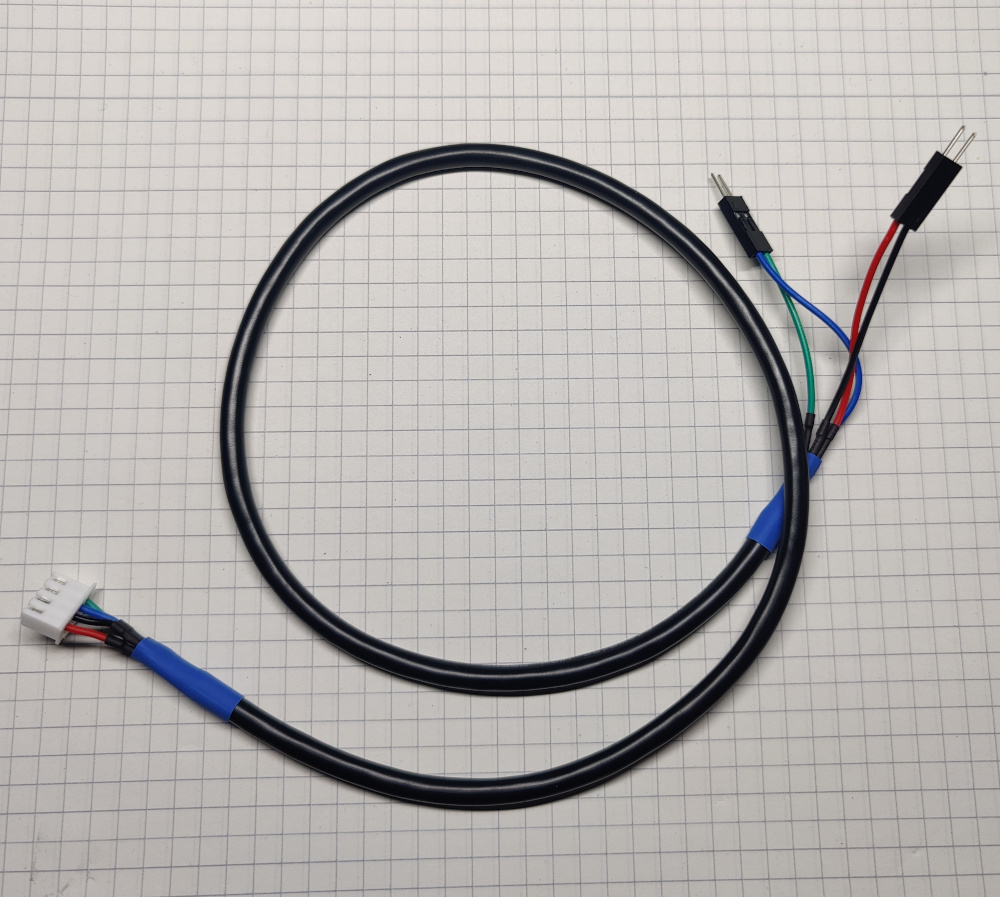
\includegraphics[width=\linewidth]{images/02_wiring/01_display_internals.jpg}
\end{minipage}

\subsubsection{Changing the level sensor plug}
\begin{minipage}[t]{0.5\linewidth}
	\vspace{0pt}
	Cut off the default plug of the A02YYUW ultrasonic sensor. Replace it with a JST-XH 4-Pin female connector. Pay attention to the color order. Don't forget shrink tubing.
\end{minipage}
\hfill
\begin{minipage}[t]{0.4\linewidth}
	\vspace{0pt}
	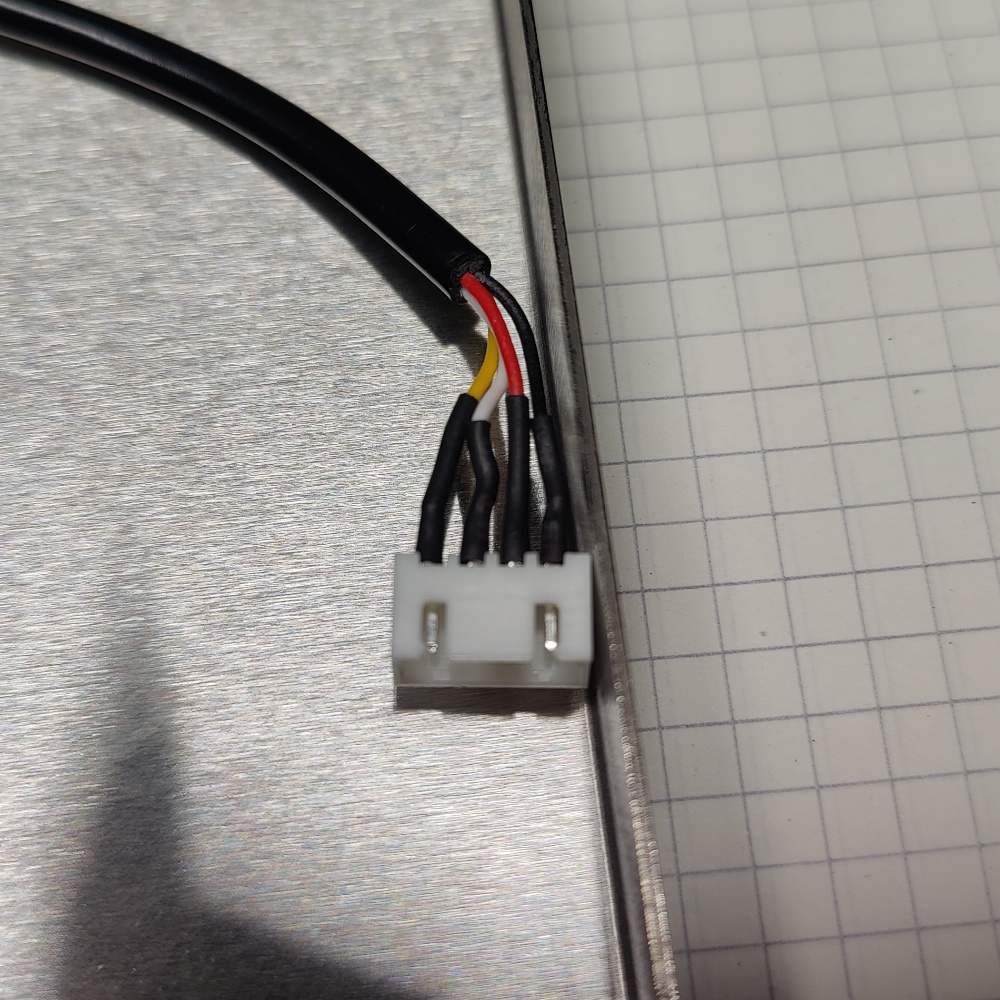
\includegraphics[width=\linewidth]{images/02_wiring/03_lid_sensor_plug.jpg}
\end{minipage}

\subsubsection{Attaching the level sensor plug}
\begin{minipage}[t]{0.5\linewidth}
	\vspace{0pt}
	Remove the water tank cover of your machine. Use the double-sided tape to stick the sensor to the bottom of the lid. Position the sensor such that it sits in the middle over the water area of the tank. For the Profitec GO, this means positioning the sensor in the middle of the lid.
\end{minipage}
\hfill
\begin{minipage}[t]{0.4\linewidth}
	\vspace{0pt}
	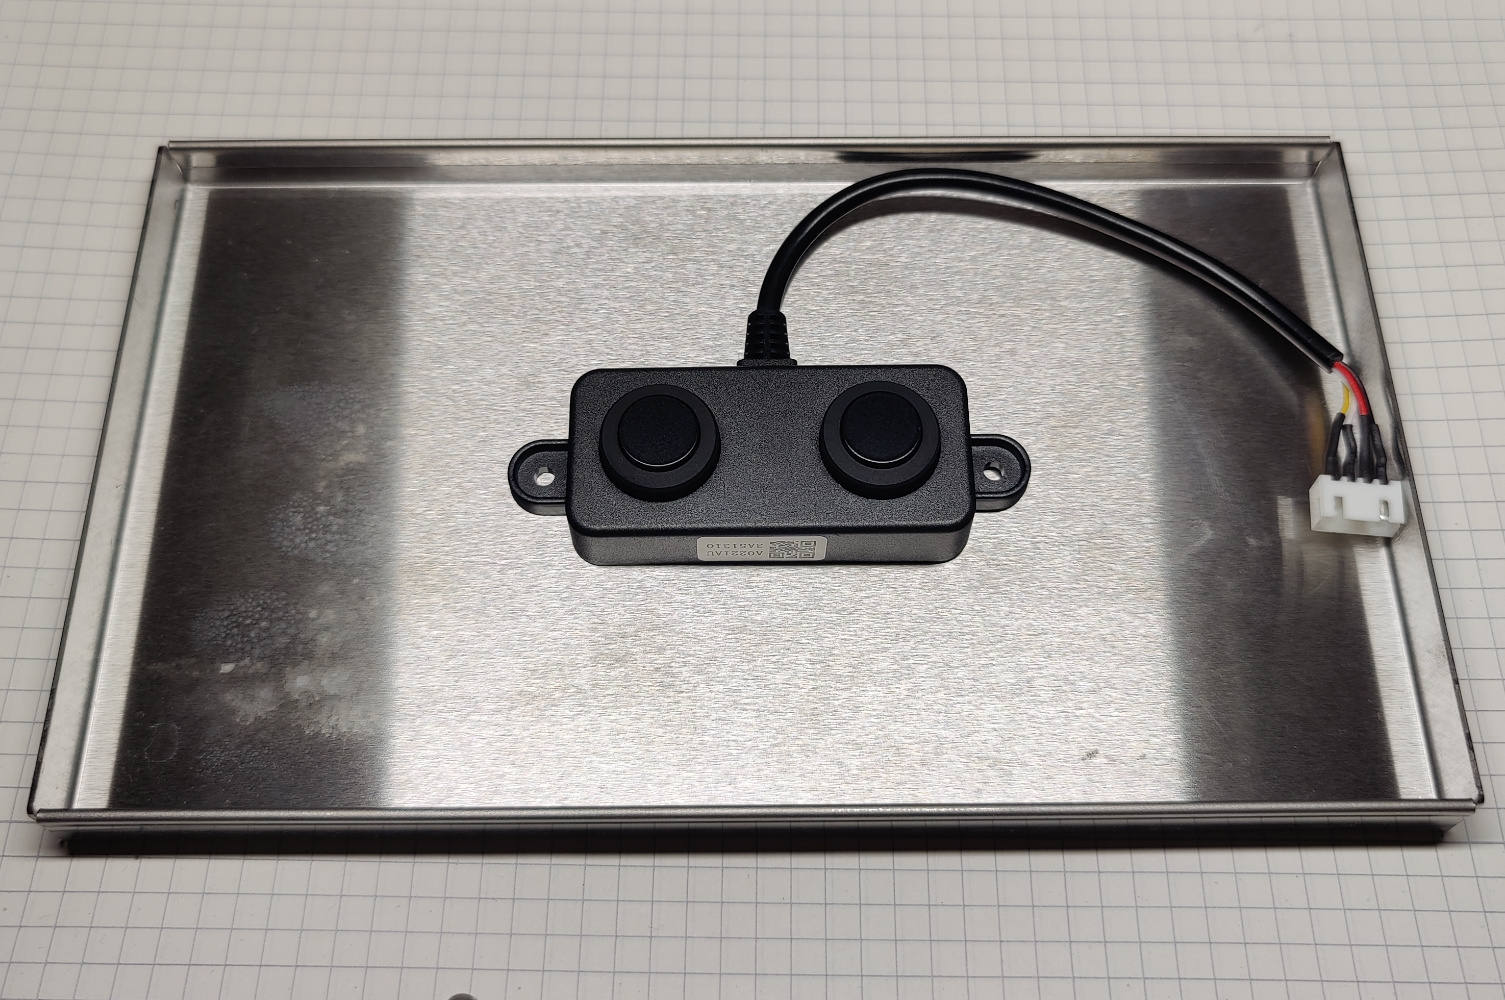
\includegraphics[width=\linewidth]{images/02_wiring/02_lid_sensor.jpg}
\end{minipage}

\subsubsection{Wiring harness}
\begin{minipage}[t]{0.5\linewidth}
	\vspace{0pt}
	Next, create a wiring harness that will connect the power supply, level sensor and the display unit. Create a Y-splitter for the red (5V) and black (ground) wires. Attach a JST-XH 2-Pin female connector to the two pole end (this will connect to the power supply). Attach a JST-XH 4-Pin male connector to one side of the 4-pole end and a 4-Pin female Dupont connector to the other 4-pole end. The 4-pole wire should be around 15cm long, the 2-pole wire around 20cm.
\end{minipage}
\hfill
\begin{minipage}[t]{0.4\linewidth}
	\vspace{0pt}
	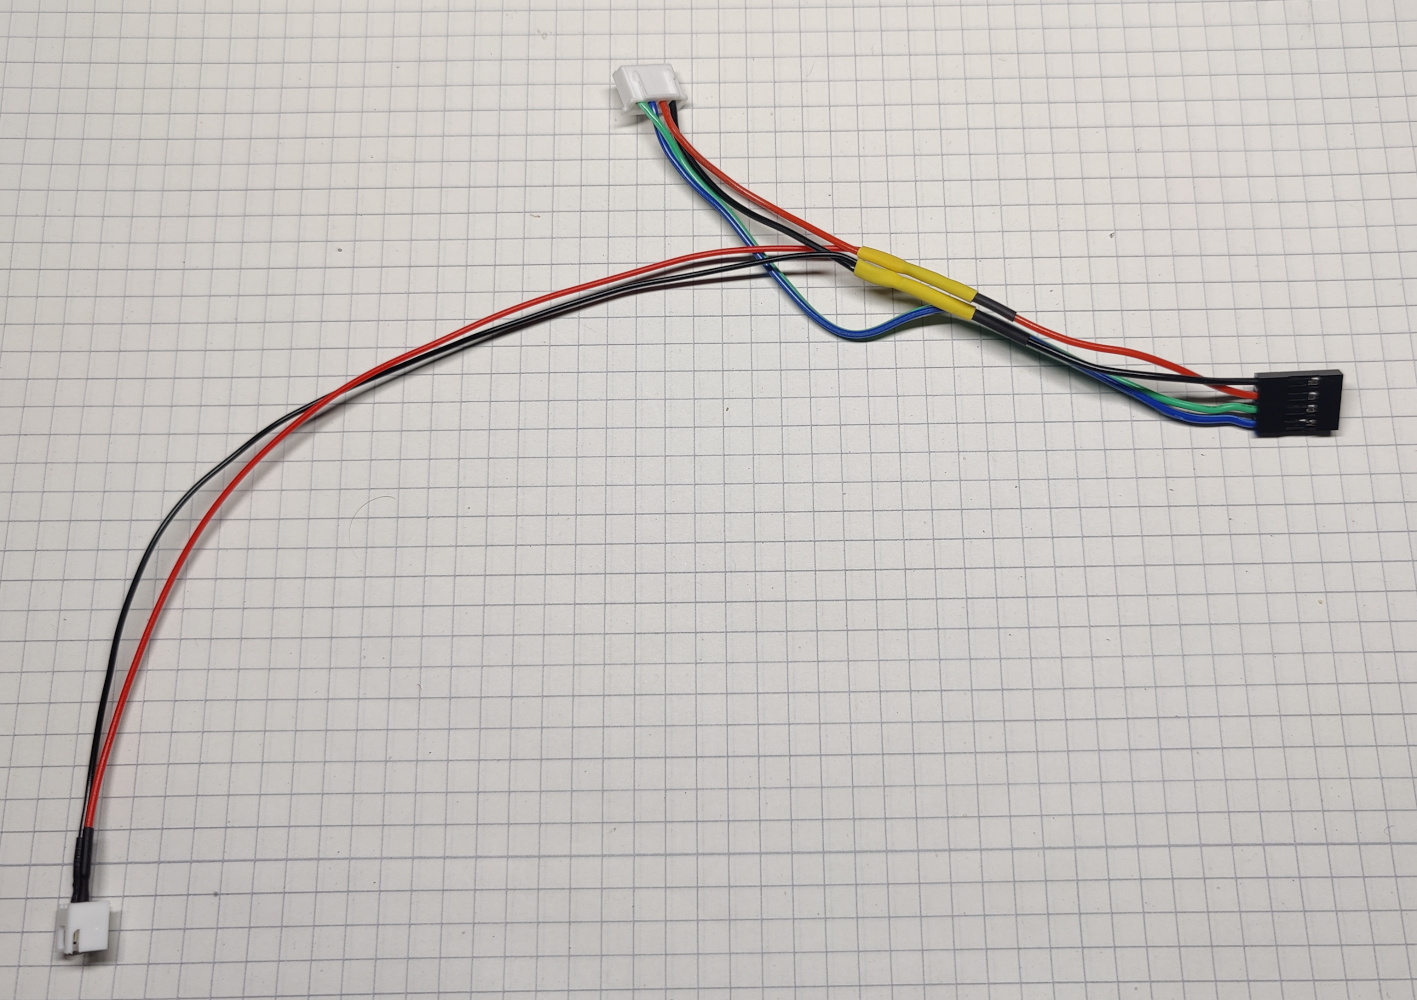
\includegraphics[width=\linewidth]{images/02_wiring/04_wiretree.jpg}
	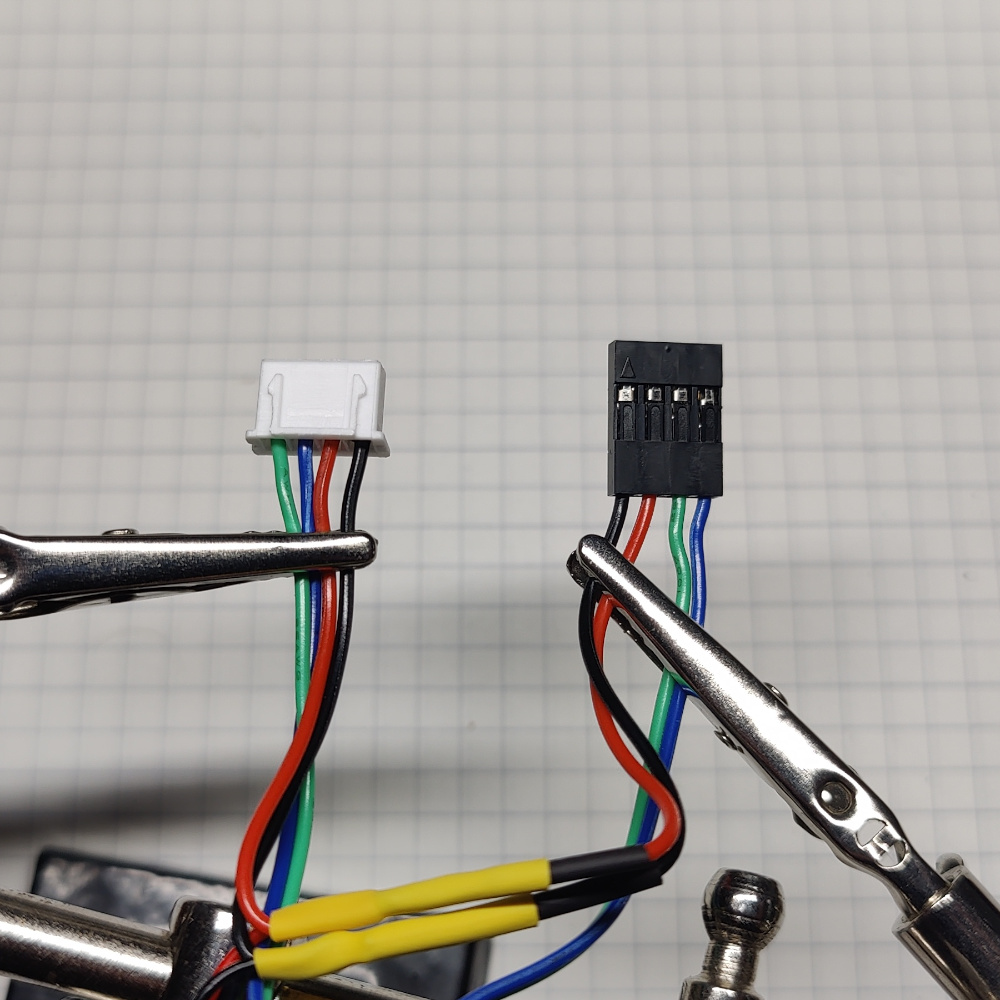
\includegraphics[width=\linewidth]{images/02_wiring/05_wiretree_plugs.jpg}
\end{minipage}

\subsubsection{Wiring harness connection check}
\begin{minipage}[t]{0.5\linewidth}
	\vspace{0pt}
	Plug the level sensor into the JST-XH 4-Pin connector of the wiring harness and plug the two 2-Pin Dupont connectors of the display cable into the 4-Pin Dupont of the wiring harness. Compare the colors of the wires to the picture to the right. Note that the blue and green wires are switched. That is because the RX-pin of the display needs to be connected to the TX-pin of the level sensor and vice-versa.
\end{minipage}
\hfill
\begin{minipage}[t]{0.4\linewidth}
	\vspace{0pt}
	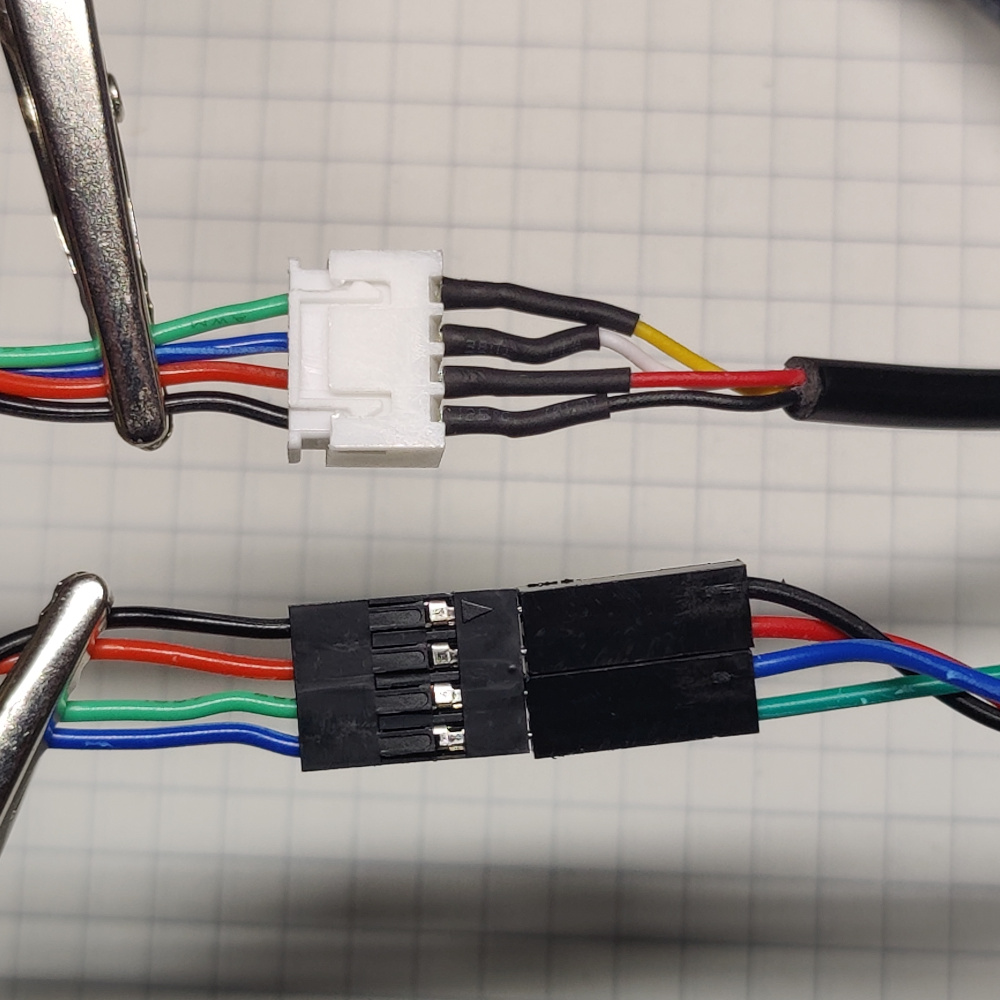
\includegraphics[width=\linewidth]{images/02_wiring/06_wiretree_plugs_connected.jpg}
\end{minipage}

\subsubsection{Power supply preparation}
\begin{minipage}[t]{0.5\linewidth}
	\vspace{0pt}
	Crimp a JST-XH 2-Pin male connector to the 5V output of your power supply. This will connect to the 2-Pin JST-XH of the wiring harness to supply the level sensor and display with power. If you want to use connectors compatible with your machine internal electronics, now is the time to crimp them to the power supply. I went with splicing connectors.
\end{minipage}
\hfill
\begin{minipage}[t]{0.4\linewidth}
	\vspace{0pt}
	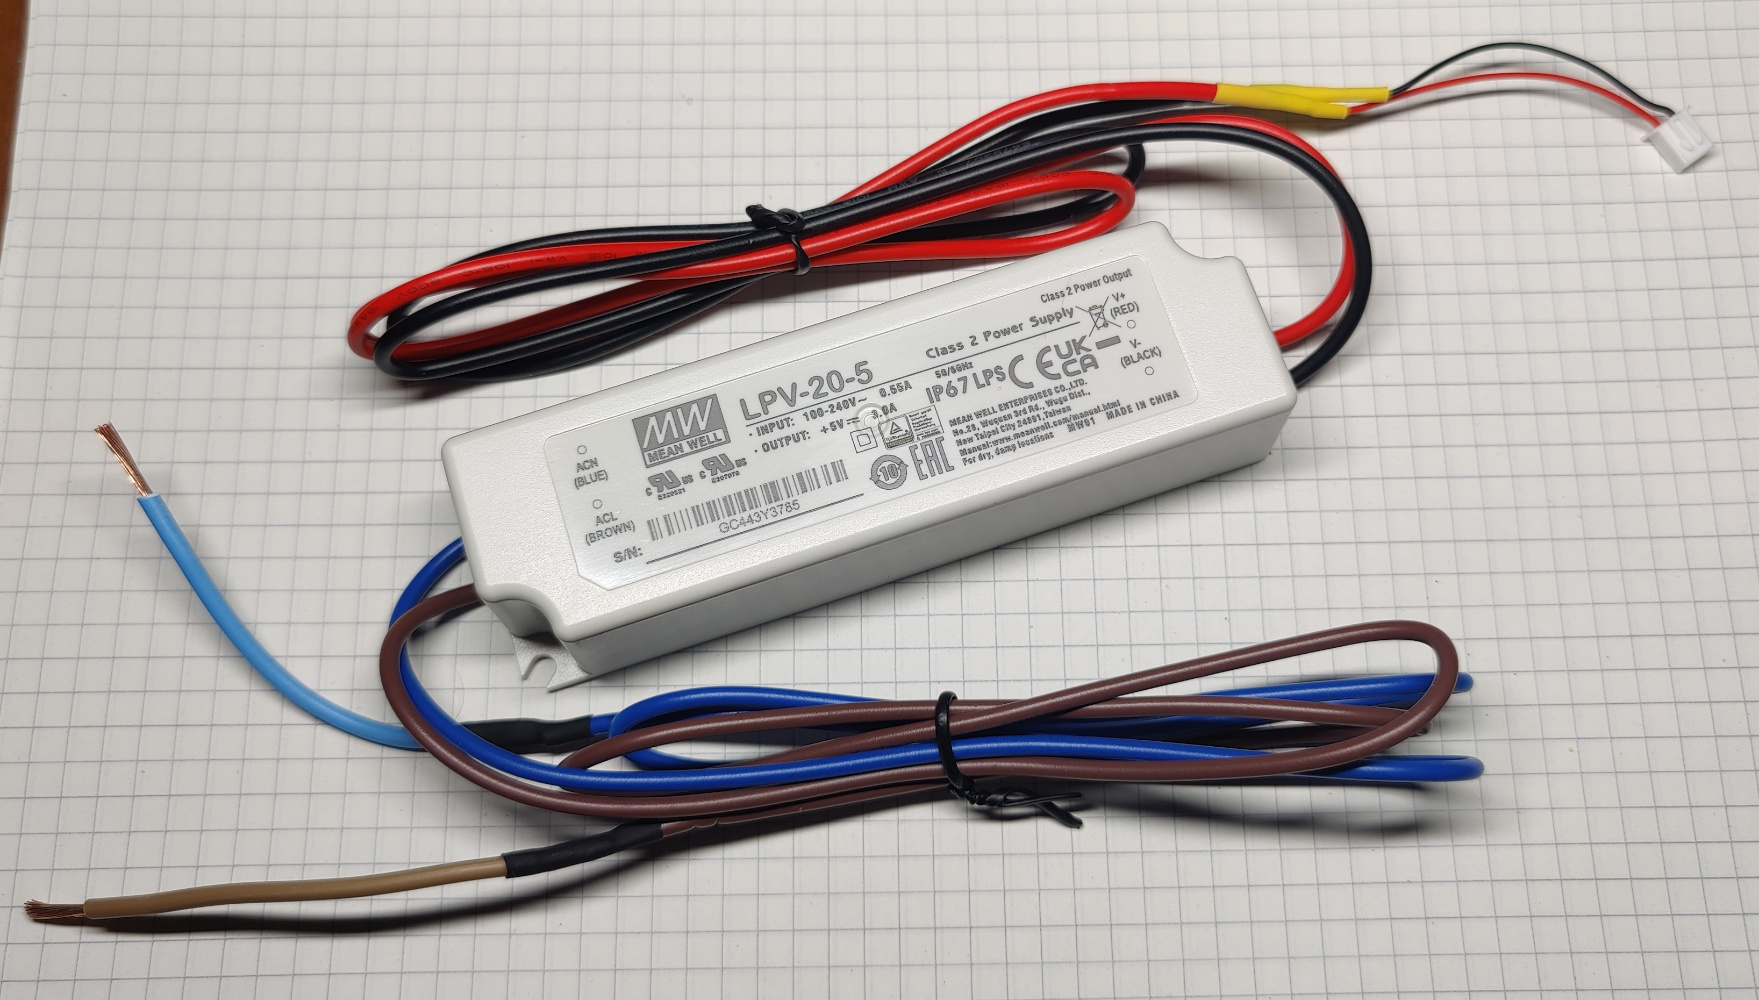
\includegraphics[width=\linewidth]{images/02_wiring/07_psu.jpg}
\end{minipage}

\subsubsection{Complete wiring overview and diagram}
\begin{minipage}[t]{0.5\linewidth}
	\vspace{0pt}
	The components connect together like shown in the picture. If you have a 5V lab power supply, feel free to power the system up to check that all connections are fine. Below is a sketch of the complete wiring. Make sure the components connect correctly.
\end{minipage}
\hfill
\begin{minipage}[t]{0.4\linewidth}
	\vspace{0pt}
	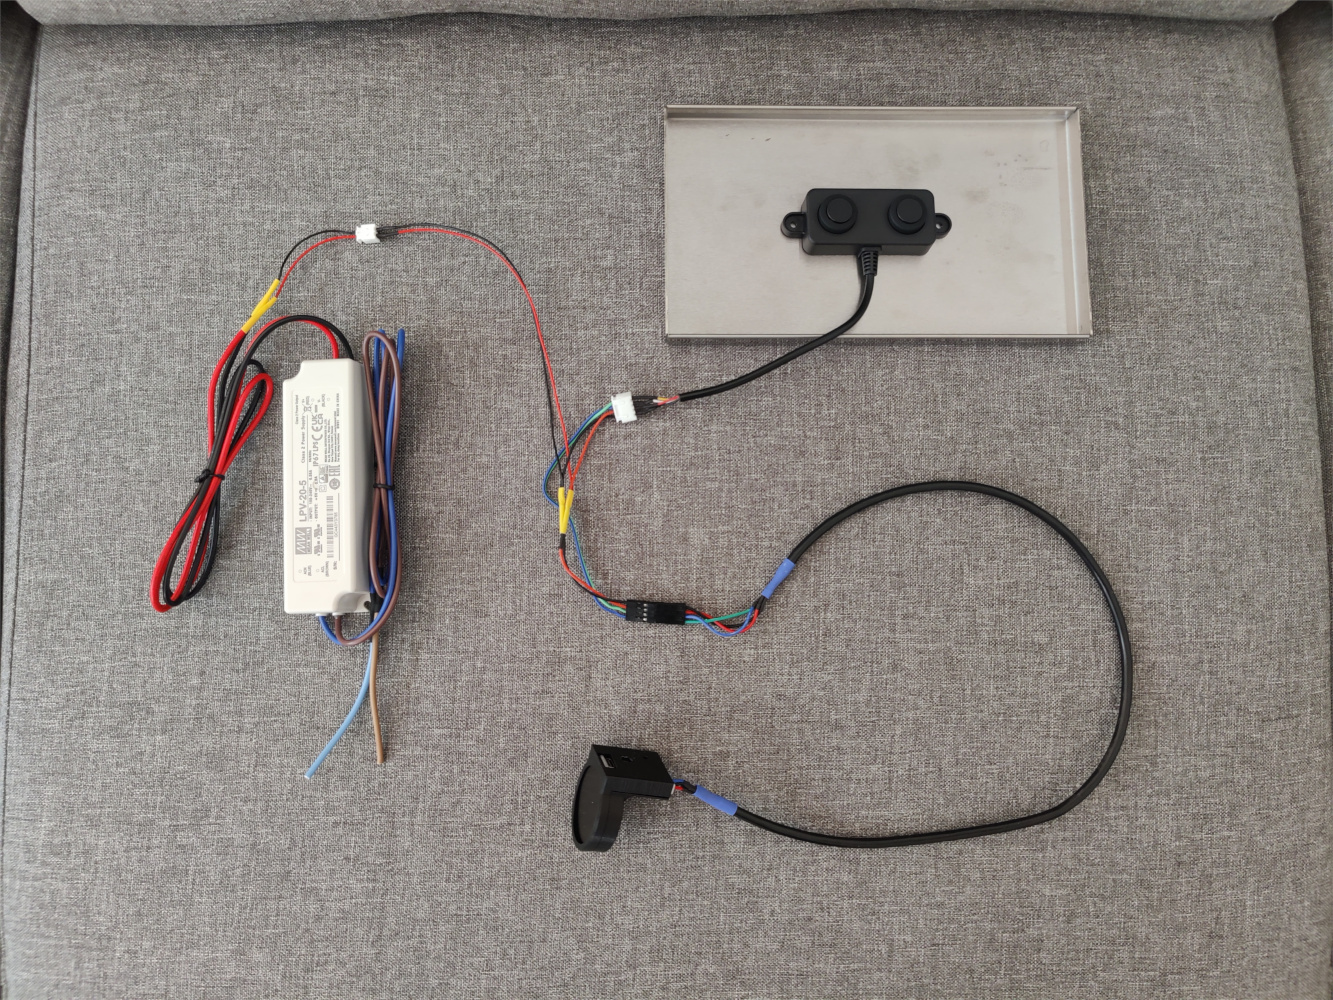
\includegraphics[width=\linewidth]{images/02_wiring/08_complete_wiring.jpg}
\end{minipage}
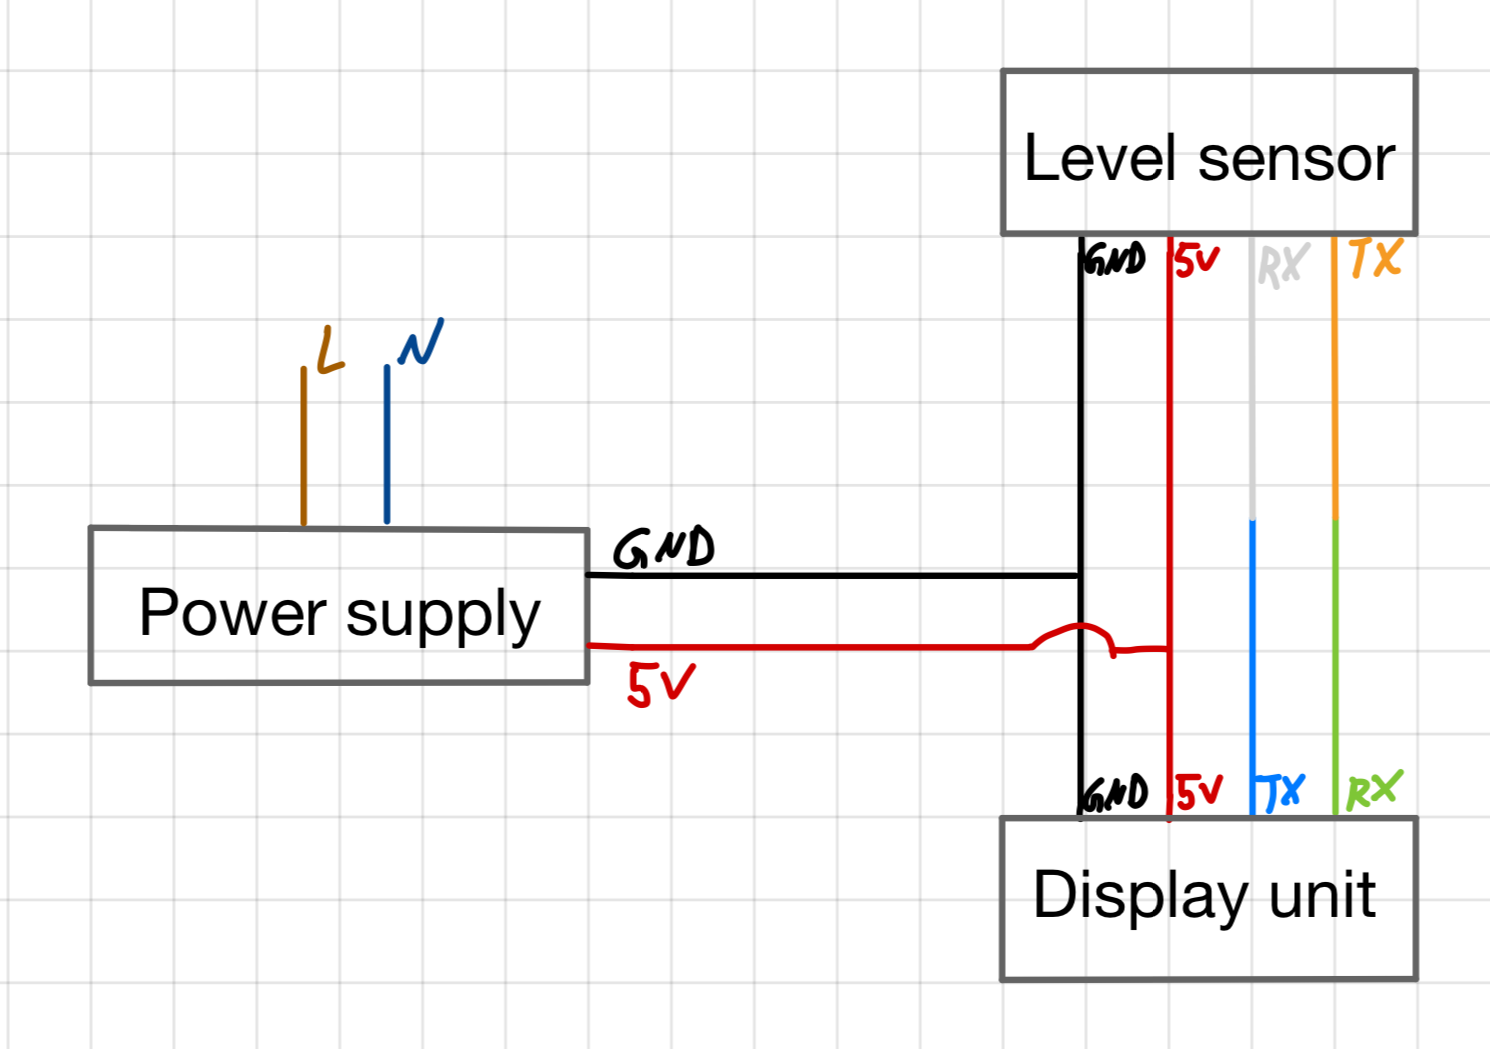
\includegraphics[width=\linewidth]{images/02_wiring/09_wiring_diagram.png}


\subsection{Machine installation}
This is your last chance to make a nice espresso before taking the machine apart. Use this opportunity to pull a shot that gets you through the remaining part of the installation :). \textbf{In this section, we will open the machine. There is the possibility to burn or shock yourself if you are not careful.} This section is specific to the Profitec GO, but you may use it as a reference for installation in a different machine.

\subsubsection{Preparation}
\begin{minipage}[t]{0.5\linewidth}
	\vspace{0pt}
	Remove the portafilter, water tray and \textbf{unplug the machine}. You may want to wait a few minutes for the machine to cool down before opening it up. 
\end{minipage}
\hfill
\begin{minipage}[t]{0.4\linewidth}
	\vspace{0pt}
	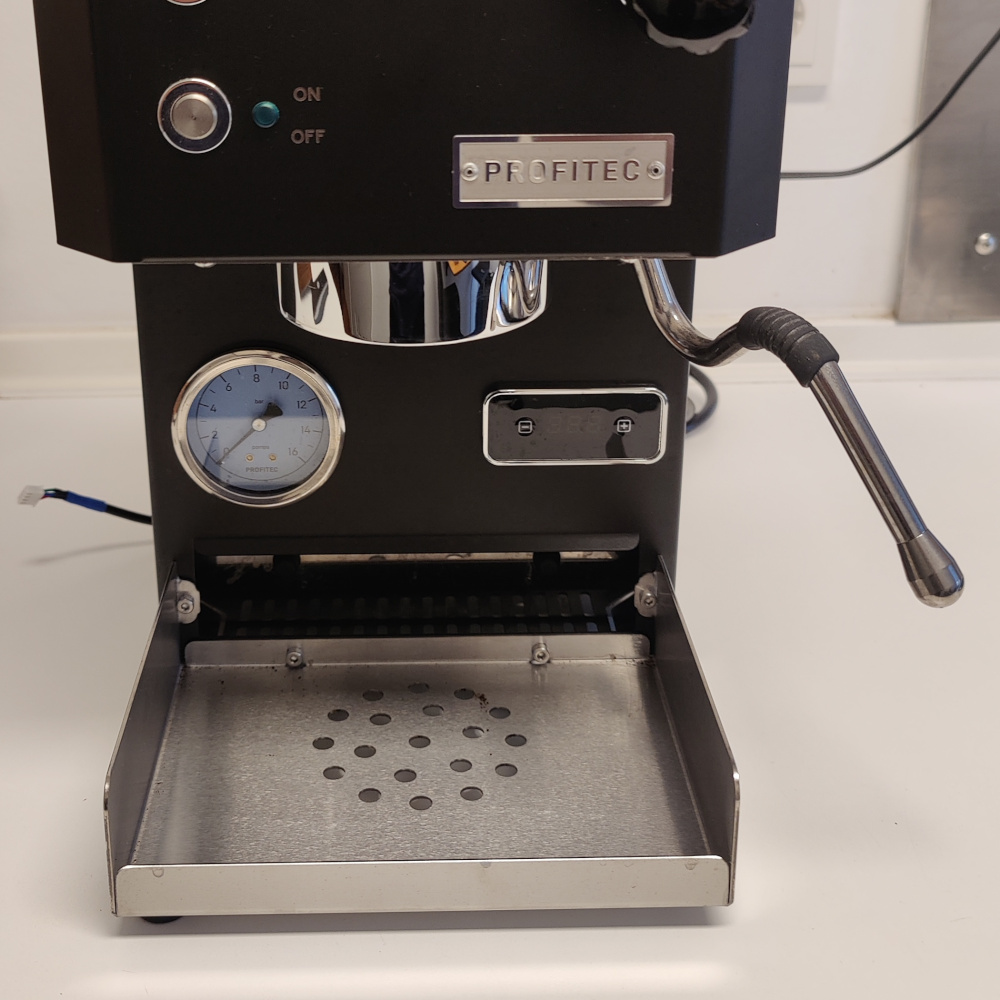
\includegraphics[width=\linewidth]{images/03_installation/01_unplug_remove.jpg}
\end{minipage}

\subsubsection{Removing the water tank}
\begin{minipage}[t]{0.5\linewidth}
	\vspace{0pt}
	Carefully pull out the water tank. When placing the water-tank onto a flat surface, I noticed that mine slowly leaks water with time. Hence, I recommend pouring the water in the tank into some other container.
\end{minipage}
\hfill
\begin{minipage}[t]{0.4\linewidth}
	\vspace{0pt}
	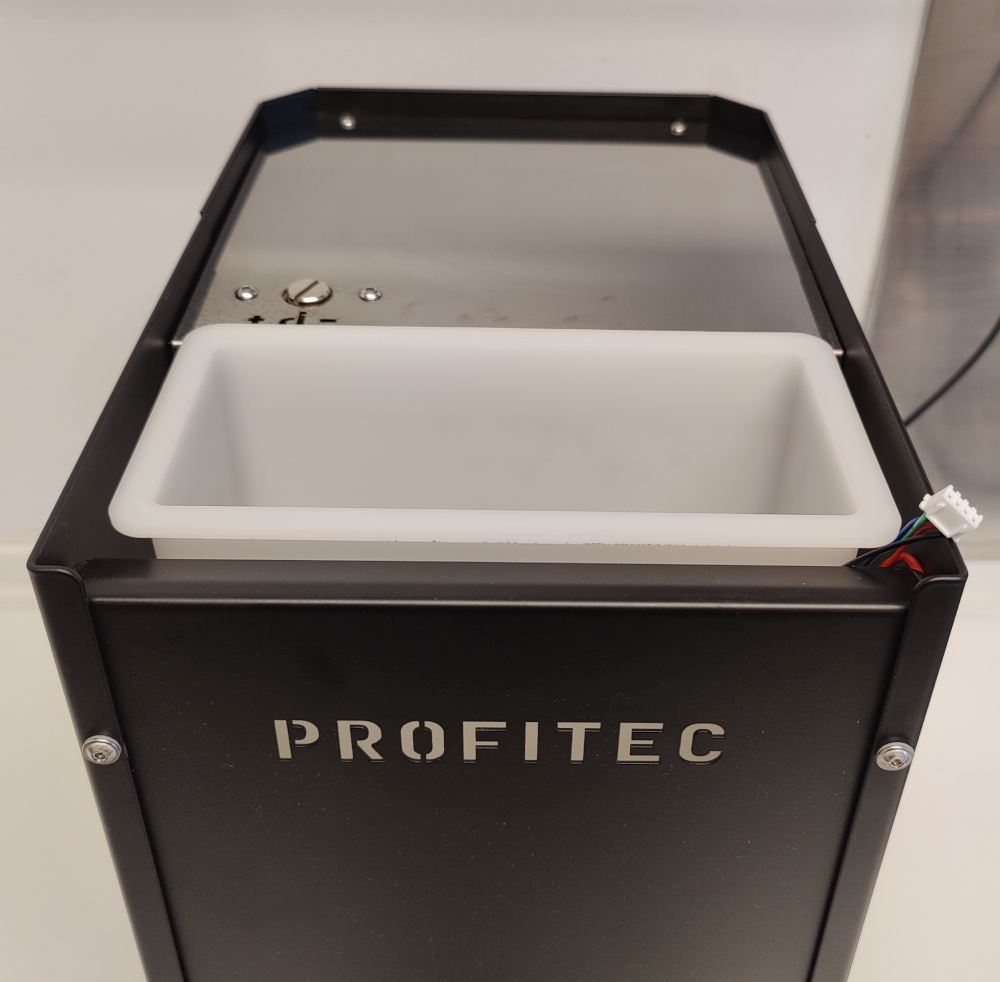
\includegraphics[width=\linewidth]{images/03_installation/02_remove_watertank.jpg}
	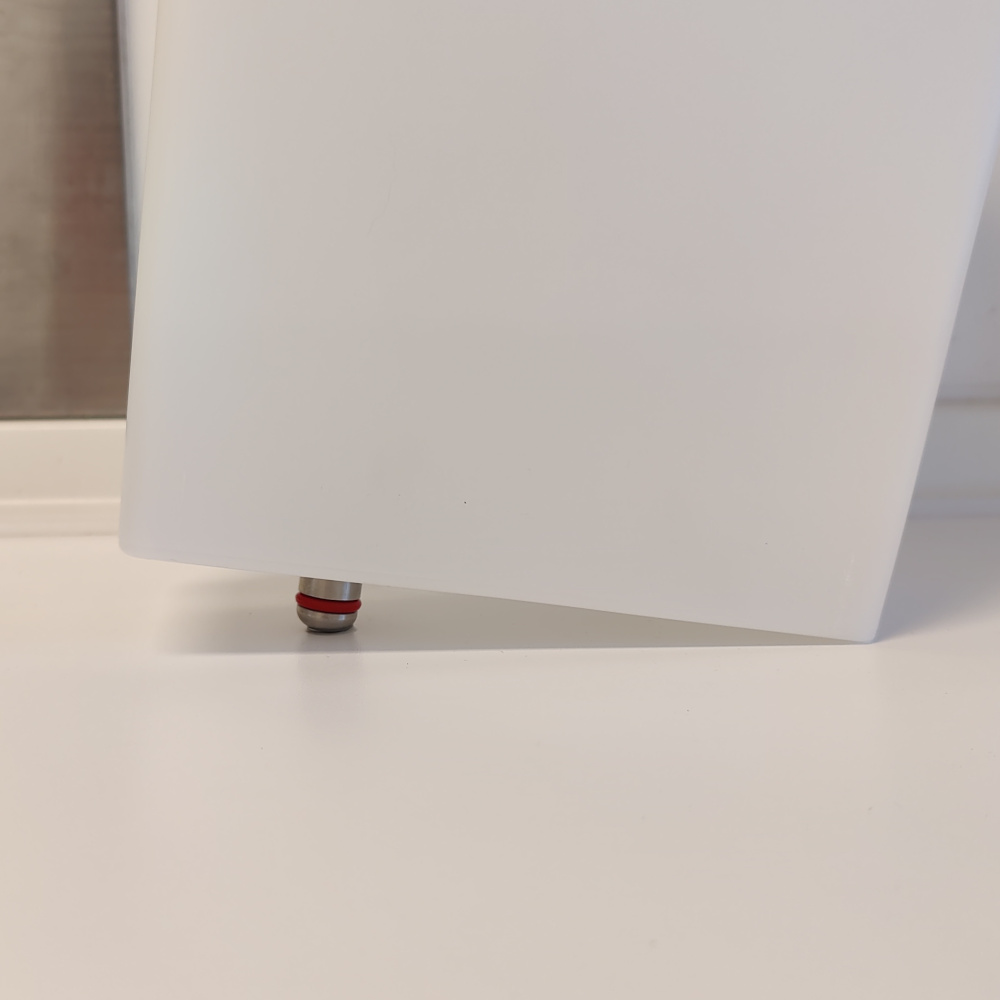
\includegraphics[width=\linewidth]{images/03_installation/03_warning_leak.jpg}
\end{minipage}

\subsubsection{Removing the backplate}
\label{sec:backplate}
\begin{minipage}[t]{0.5\linewidth}
	\vspace{0pt}
	\textbf{Verify that the machine is unplugged!} Unscrew the six screws on the back of the machine. Slide the backplate out upwards. Place it on some soft surface (e.g. a towel) to avoid scratches. Do NOT place any other parts we are about to remove on top of it.
\end{minipage}
\hfill
\begin{minipage}[t]{0.4\linewidth}
	\vspace{0pt}
	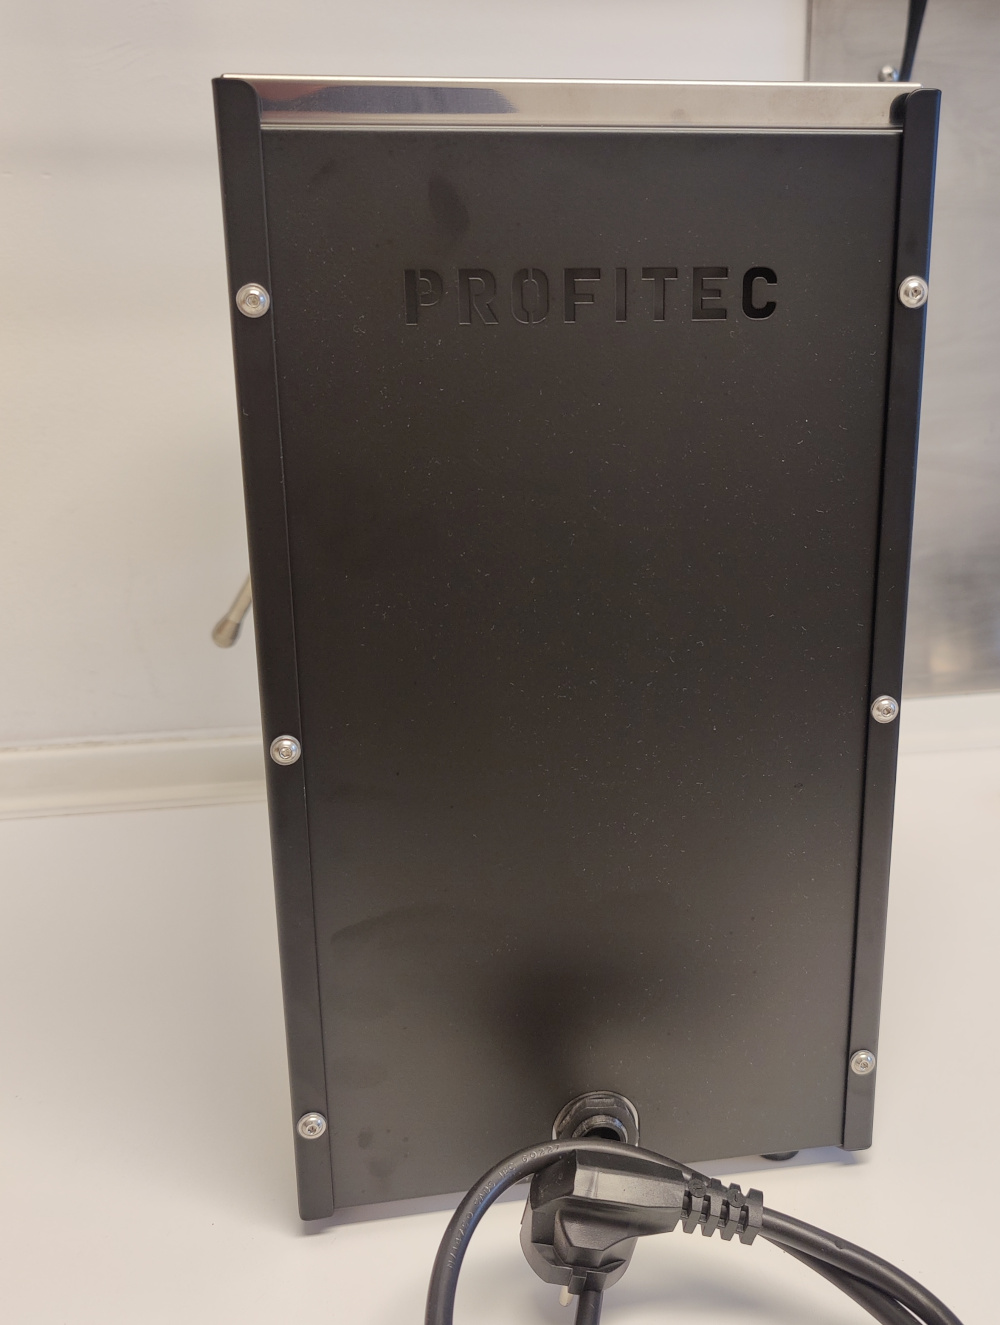
\includegraphics[width=\linewidth]{images/03_installation/04_remove_screws_check_unplug.jpg}
\end{minipage}

\subsubsection{Removing the topplate}
\label{sec:topplate}
\begin{minipage}[t]{0.5\linewidth}
	\vspace{0pt}
	Unscrew the six screws securing the topplate. Lift it up to remove it. Place it on some soft surface (e.g. a towel) to avoid scratches. Do NOT place any other parts we are about to remove on top of it. The boiler is located below, which may be still hot. Be careful not to burn yourself.
\end{minipage}
\hfill
\begin{minipage}[t]{0.4\linewidth}
	\vspace{0pt}
	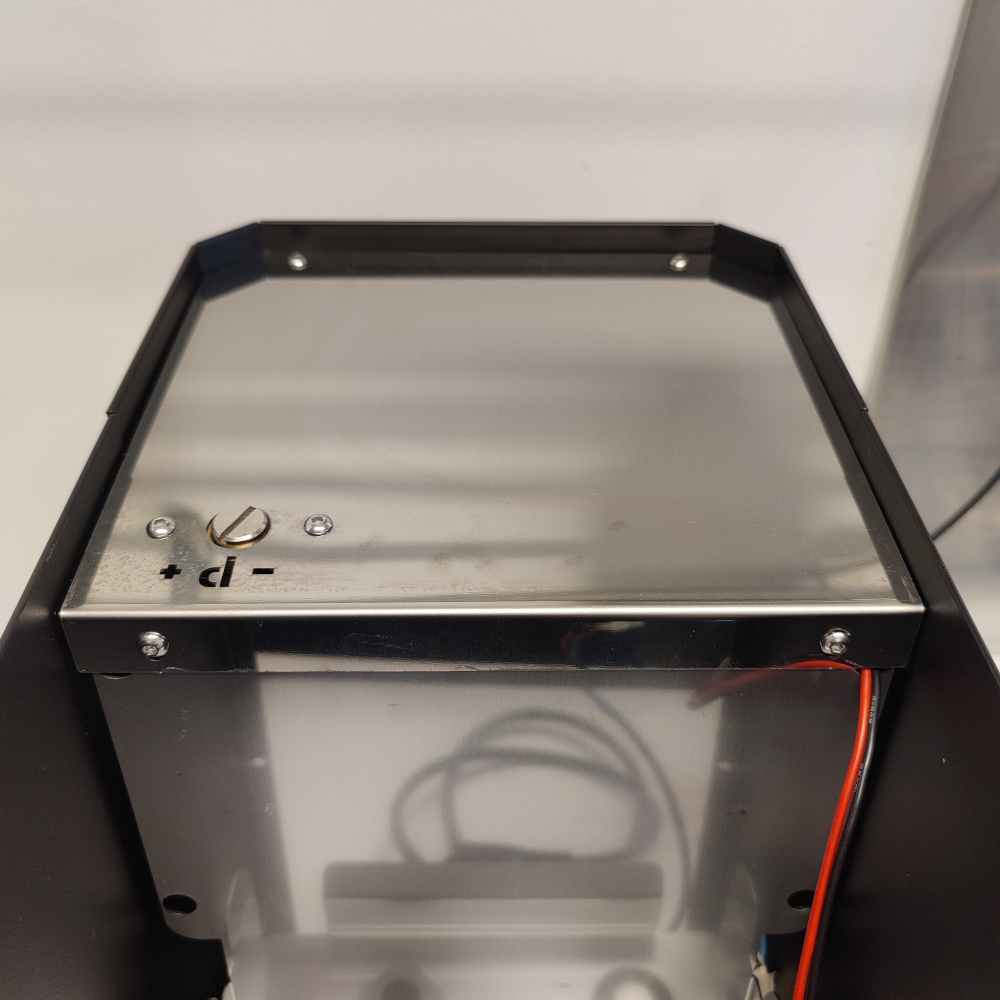
\includegraphics[width=\linewidth]{images/03_installation/05_remove_top.jpg}
\end{minipage}

\subsubsection{Removing the dividerplate}
\label{sec:dividerplate}
\begin{minipage}[t]{0.5\linewidth}
	\vspace{0pt}
	Next, we have to remove the divider that separates the water-tank from the electronics. This is a bit tricky, since the screws are located at the bottom of the machine. There are two screws that need to be removed, highlighted in the first picture. If you are alone, I recommend positioning the machine at the edge of the table and slightly tilting it, until you can unscrew it from the bottom (shown in second picture). Once the screws on both sides are out, you also need to unscrew the water intake (third picture). Afterwards, carefully slide the dividerplate out. Place it on some soft surface (e.g. a towel) to avoid scratches. Do NOT place any other parts we are about to remove on top of it. Do not damage any of the waterlines or cables! The intake may have some remaining water, take a piece of papertowel to drain it (fourth picture).
\end{minipage}
\hfill
\begin{minipage}[t]{0.4\linewidth}
	\vspace{0pt}
	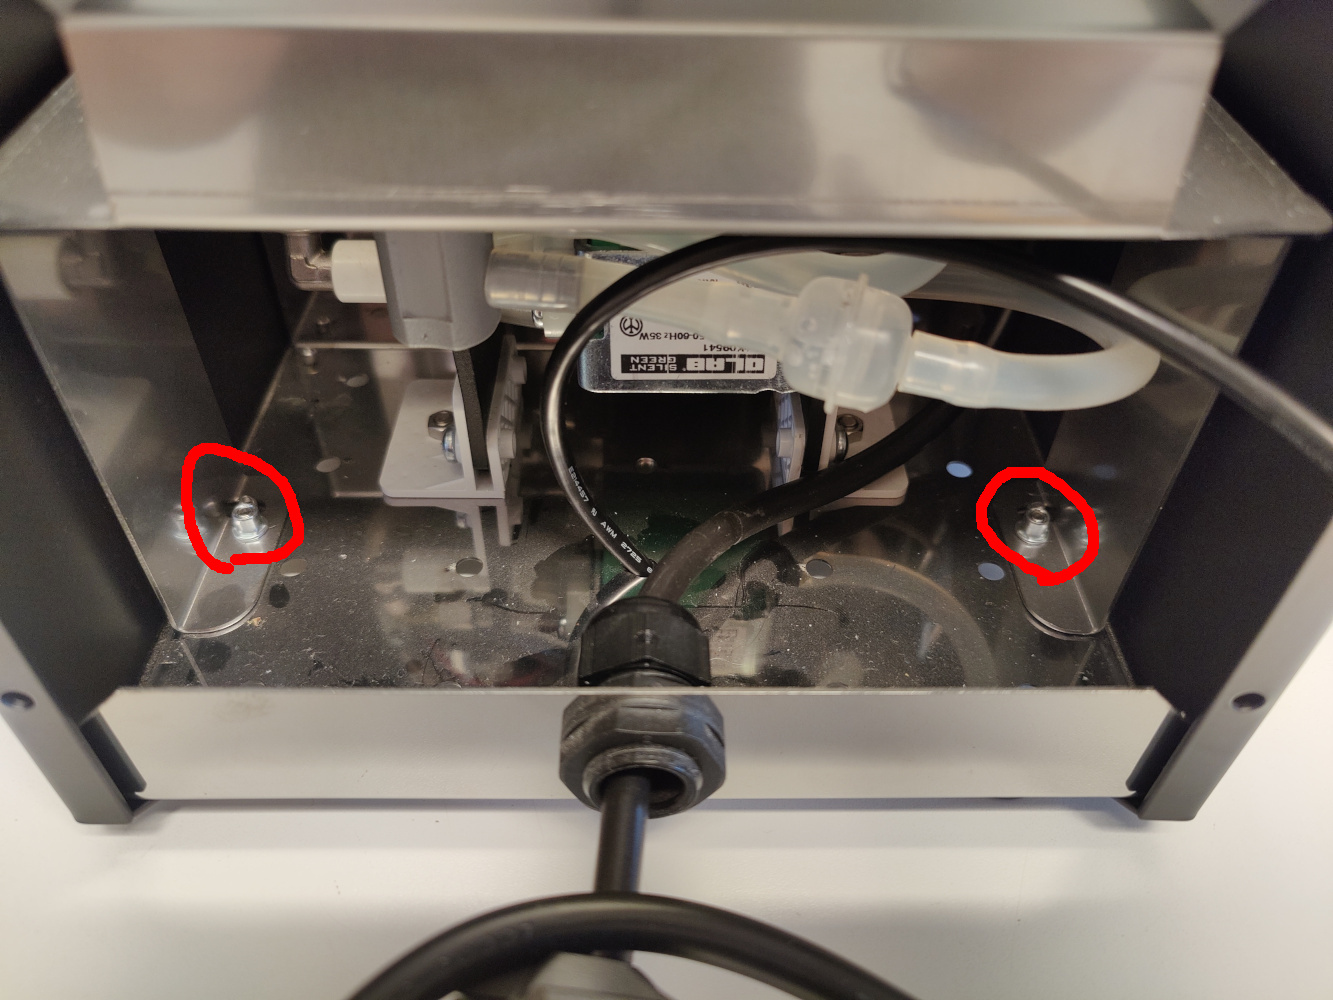
\includegraphics[width=\linewidth]{images/03_installation/06_remove_divider_screws1.jpg}
	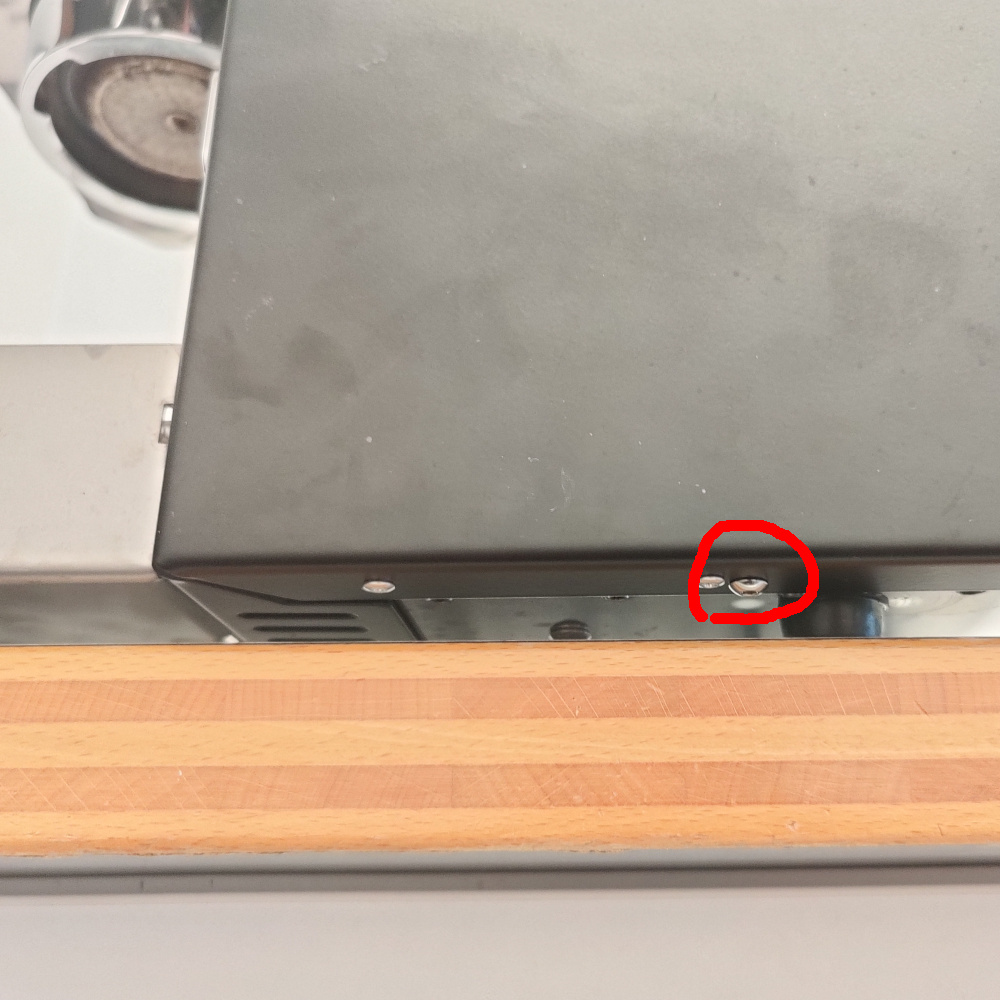
\includegraphics[width=\linewidth]{images/03_installation/07_remove_divider_screws2.jpg}
	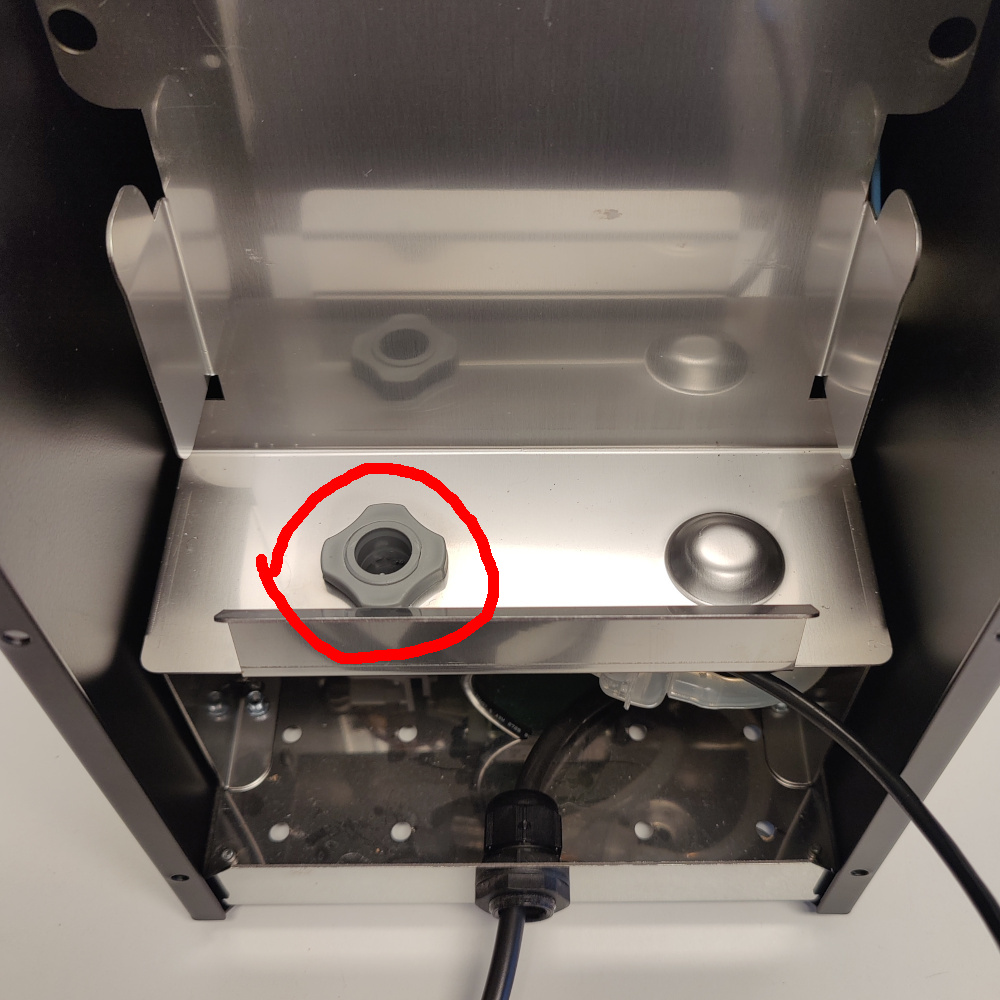
\includegraphics[width=\linewidth]{images/03_installation/08_remove_waterplug_screw.jpg}
	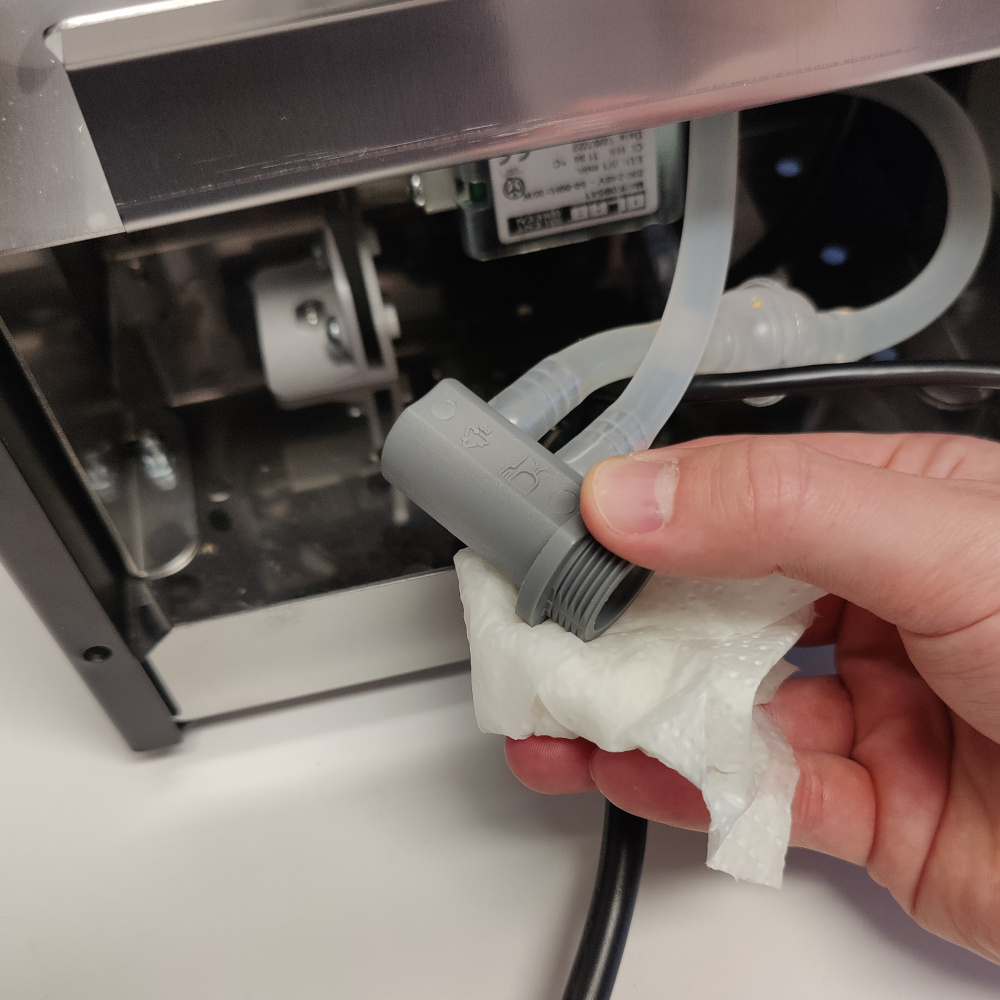
\includegraphics[width=\linewidth]{images/03_installation/09_drain_water.jpg}
\end{minipage}

\subsubsection{Pulling through the display cable}
\begin{minipage}[t]{0.5\linewidth}
	\vspace{0pt}
	Take the display cable and push the end with the two 2-Pin connectors through one of the holes at the bottom of the machine. The connectors need to be passed through one after the other in order to fit through the hole. You can plug in the display unit at the other end and stick it to the location you would like to have it. That way, you know exactly how much cable you need to leave hanging out.
\end{minipage}
\hfill
\begin{minipage}[t]{0.4\linewidth}
	\vspace{0pt}
	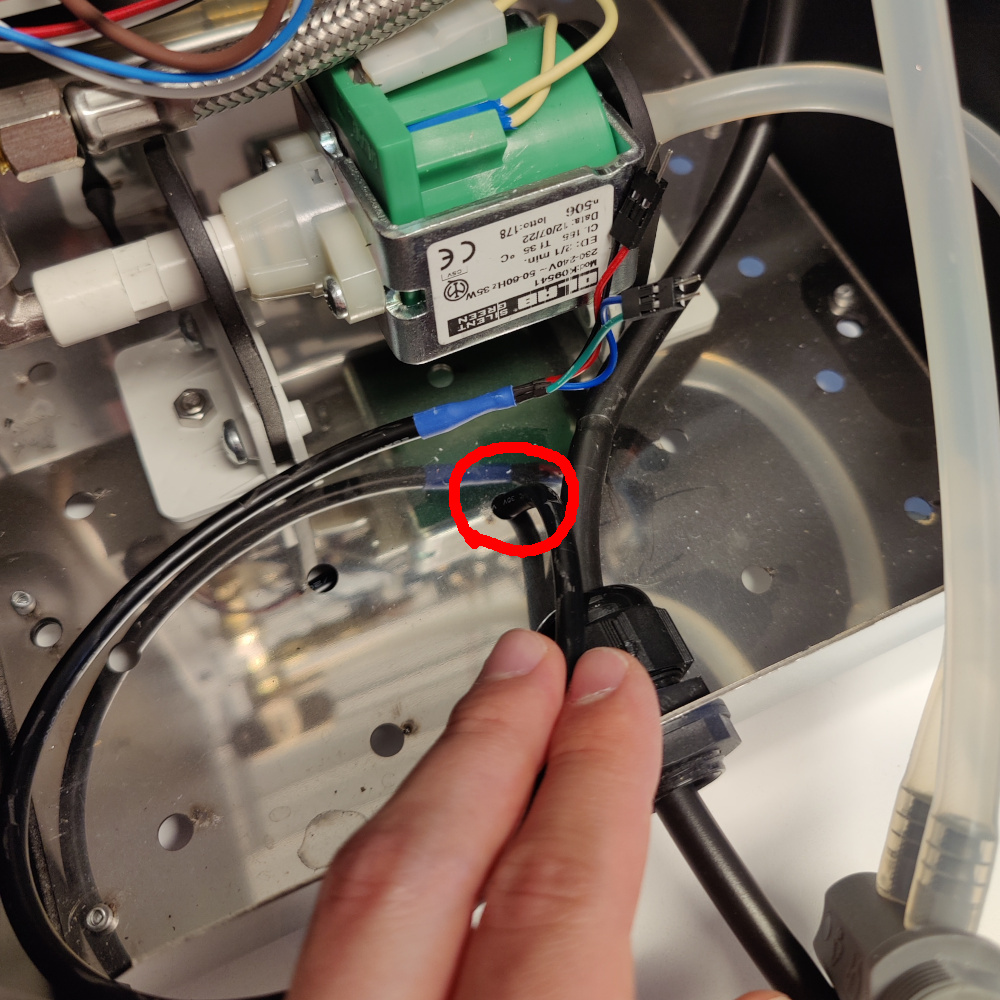
\includegraphics[width=\linewidth]{images/03_installation/10_push_through_cable.jpg}
\end{minipage}

\subsubsection{Connecting the power supply}
\begin{minipage}[t]{0.5\linewidth}
	\vspace{0pt}
	\textbf{Check again that the machine is unplugged!} In this step, we have to connect the power supply to the mains voltage, so ideally there shouldn't be any live wires. Connecting the power supply can be done in a non-destructive way by building adapters for the plugs used in your machine. The method I went with is destructive and splices open the power cord. To do this, unscrew the black cap at the power cord inlet to be able to pull the power cord through the hole and give you better access to the cord. Mark about 5cm with two pieces of tape (first image). Remove the outer isolation between the two pieces of tape (second image). \textbf{Be careful not to damage the inner isolation of the three wires}. There is a blue, brown and green-yellow cable inside. Cut the blue and brown wire in the middle. \textbf{Do NOT cut the yellow-green wire. Its purpose is to prevent the machine from killing you.} Strip some of the isolation off and reconnect them using splicing connectors (third picture). I am using WAGO connectors, which need 11mm if isolation removed from the end. Use the third port in each connector to connect the power supply (fourth picture).
\end{minipage}
\hfill
\begin{minipage}[t]{0.4\linewidth}
	\vspace{0pt}
	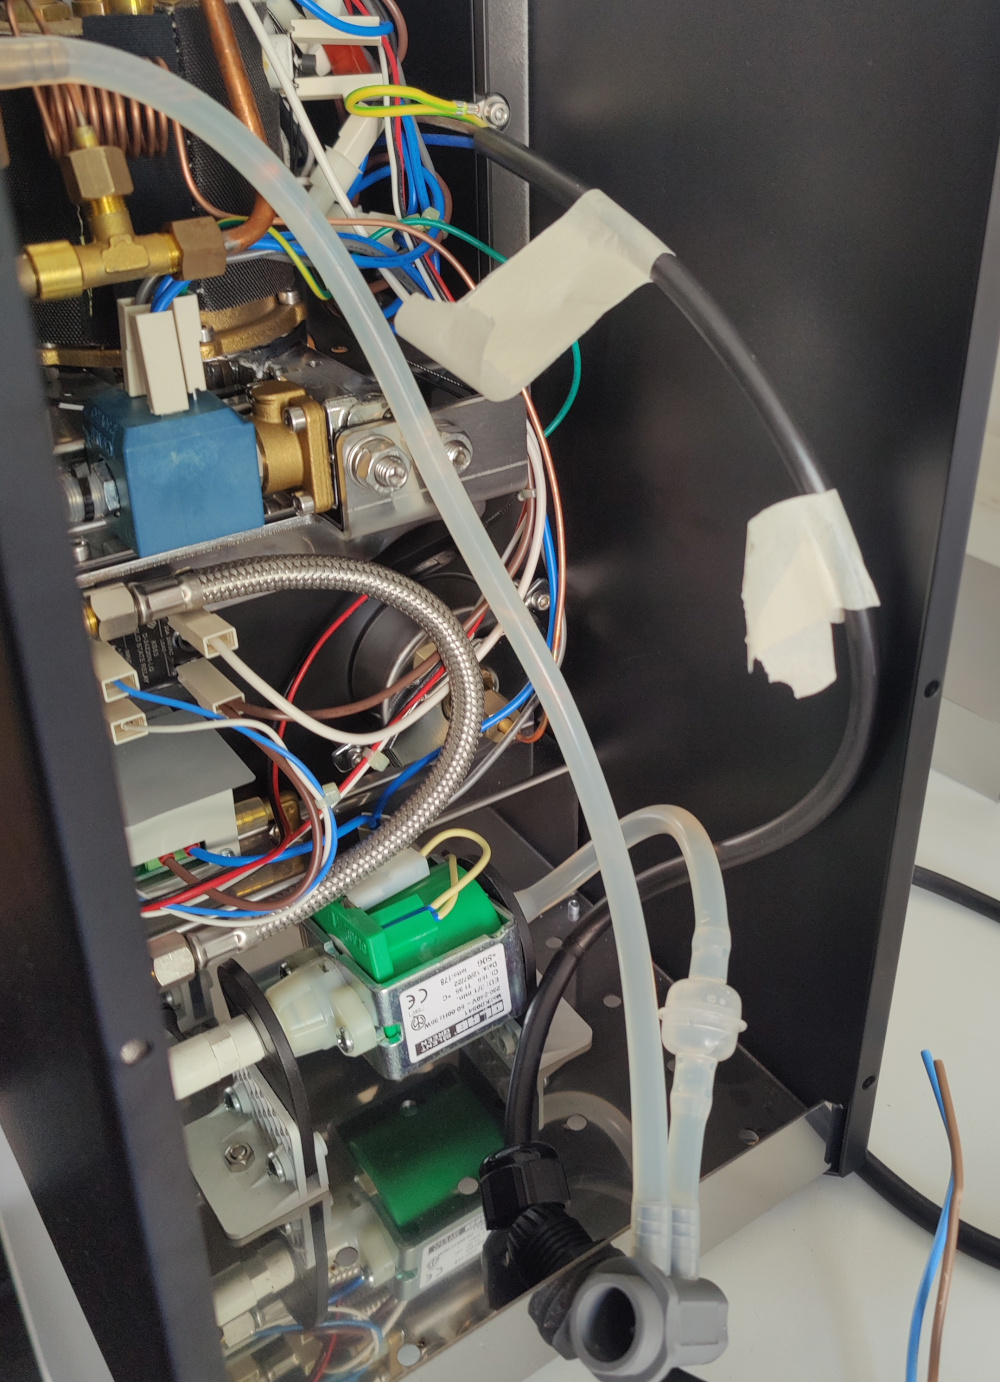
\includegraphics[width=\linewidth]{images/03_installation/11_unscrew_eucableclamp_mark_cutting.jpg}
	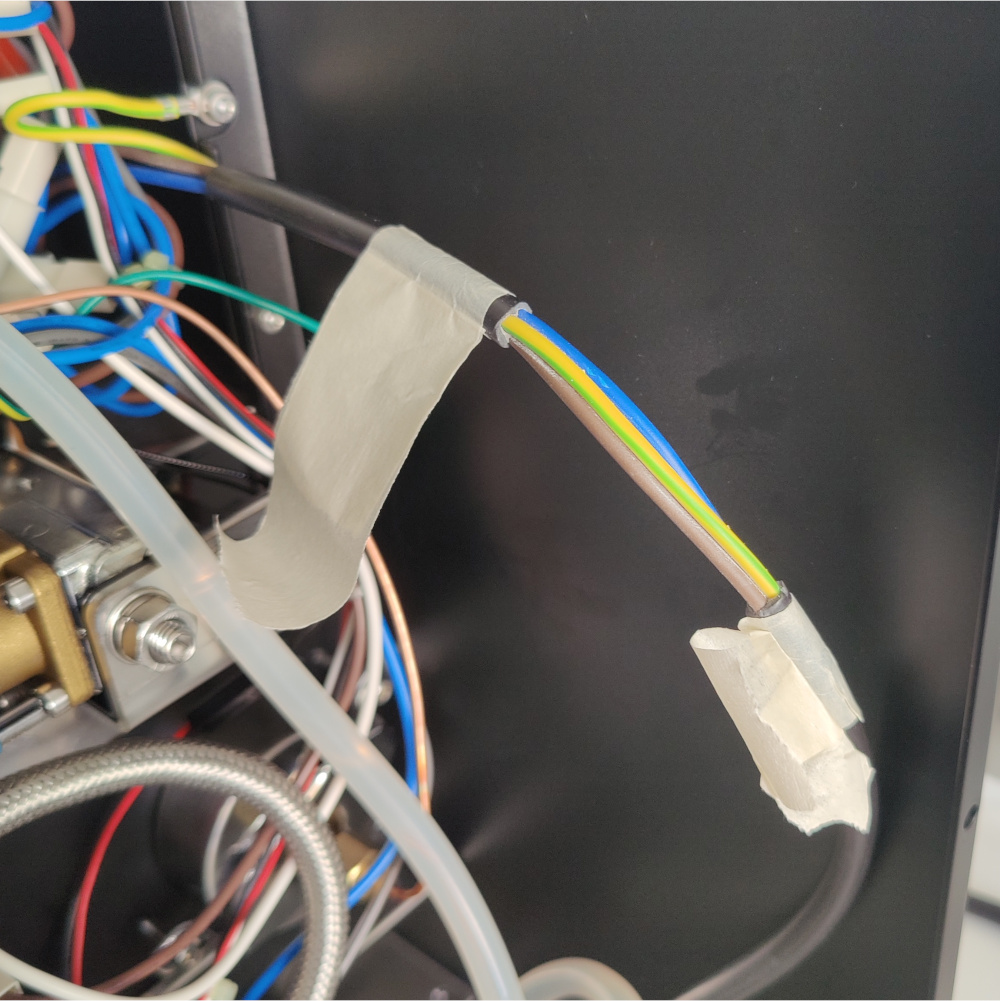
\includegraphics[width=\linewidth]{images/03_installation/12_remove_shielding.jpg}
	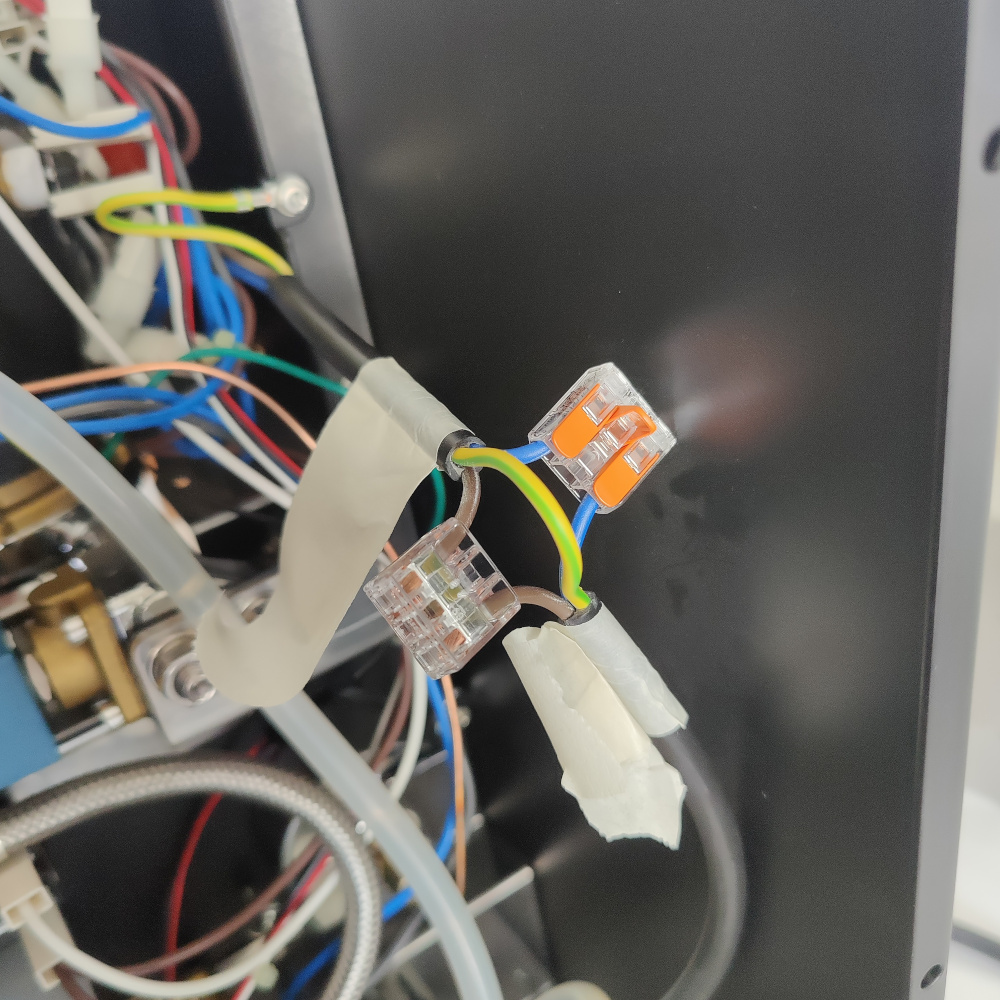
\includegraphics[width=\linewidth]{images/03_installation/13_cut_strip_wago.jpg}
	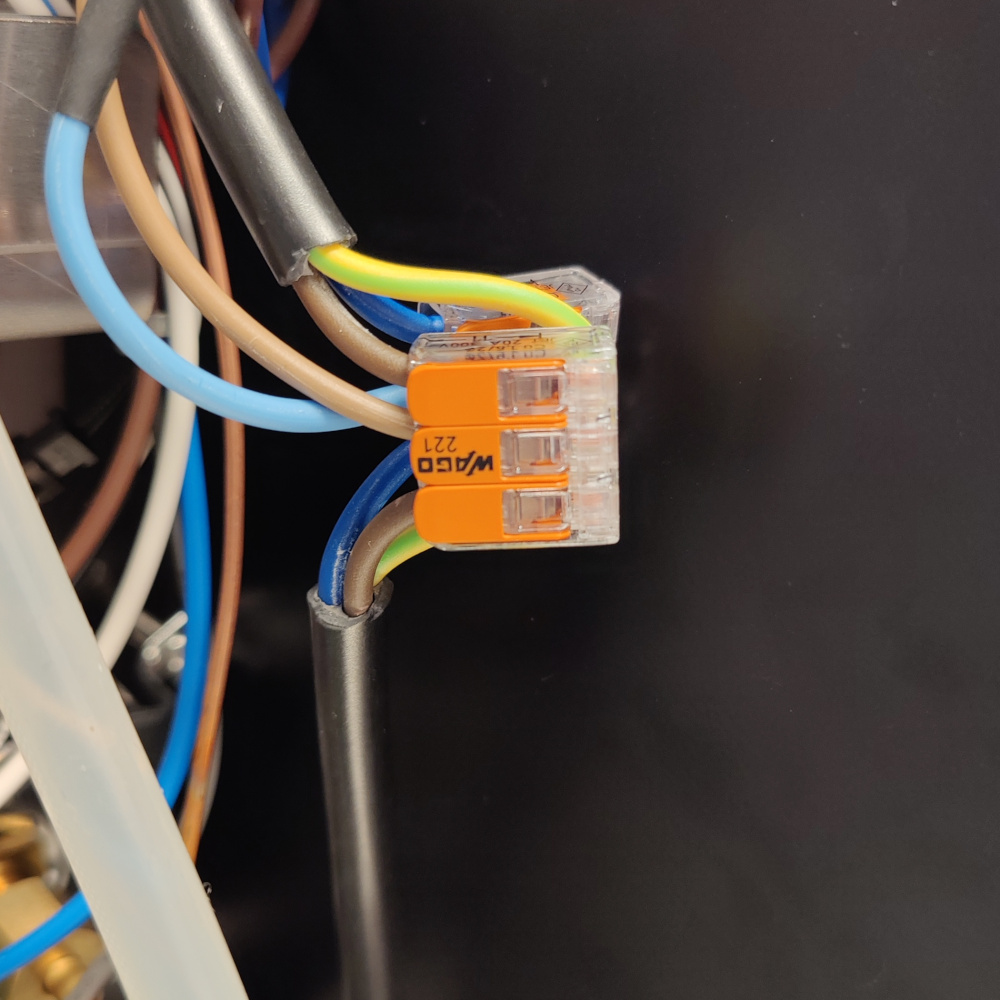
\includegraphics[width=\linewidth]{images/03_installation/14_connect_psu.jpg}
\end{minipage}

\subsubsection{Installing the power supply and dividerplate}
\begin{minipage}[t]{0.5\linewidth}
	\vspace{0pt}
	Use the double-sided tape to stick the power supply to the side of the machine like shown in the picture. If you are unsure where exactly to position it, take the dividerplate and topplate to figure out how much space you have and where to install the power supply without interference. Reinstall the dividerplate by performing the steps in Section~\ref{sec:dividerplate} in reverse.
\end{minipage}
\hfill
\begin{minipage}[t]{0.4\linewidth}
	\vspace{0pt}
	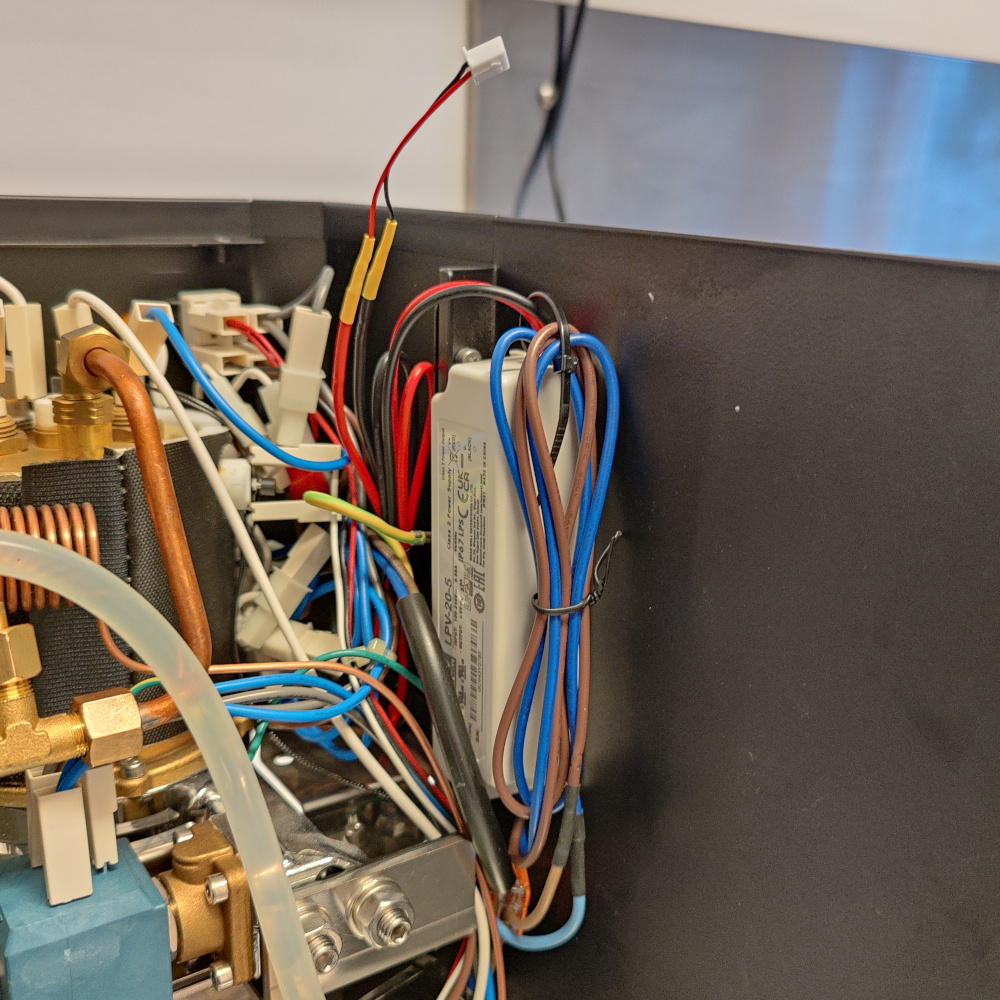
\includegraphics[width=\linewidth]{images/03_installation/15_stick_psu_to_machine_reinstall_divider.jpg}
\end{minipage}

\subsubsection{Installing the topplate}
\begin{minipage}[t]{0.5\linewidth}
	\vspace{0pt}
	Take the wire harness and thread the 2-Pin JST-XH connector of the wire harness through the hole in the divider plate. Connect it to the power supply. Reinstall the topplate by performing the steps in Section~\ref{sec:topplate} in reverse. Do not fully tighten all screws of the topplate directly! First, screw all of them in loose, then one by one tighten them to avoid any tension building up across the plate. Make sure the two wires running through the hole aren't pinched.
\end{minipage}
\hfill
\begin{minipage}[t]{0.4\linewidth}
	\vspace{0pt}
	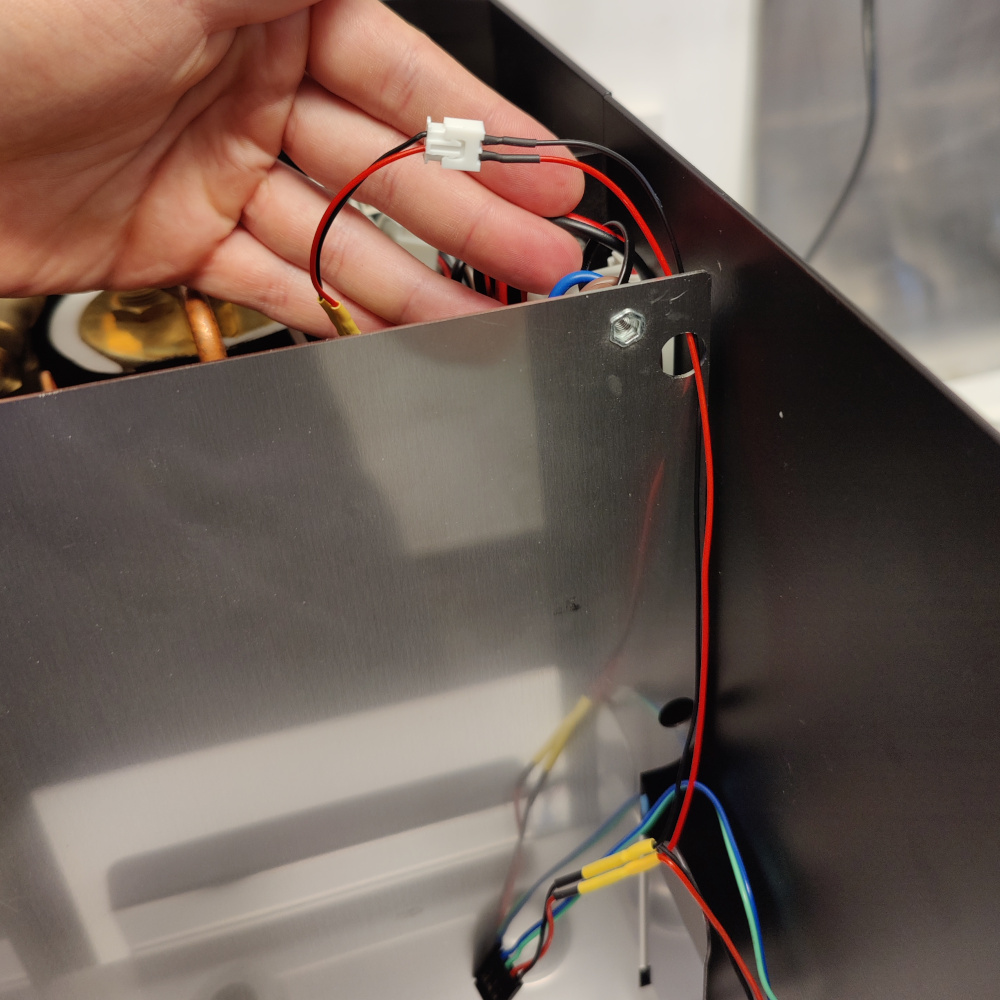
\includegraphics[width=\linewidth]{images/03_installation/16_connect_wiretree_psu.jpg}
	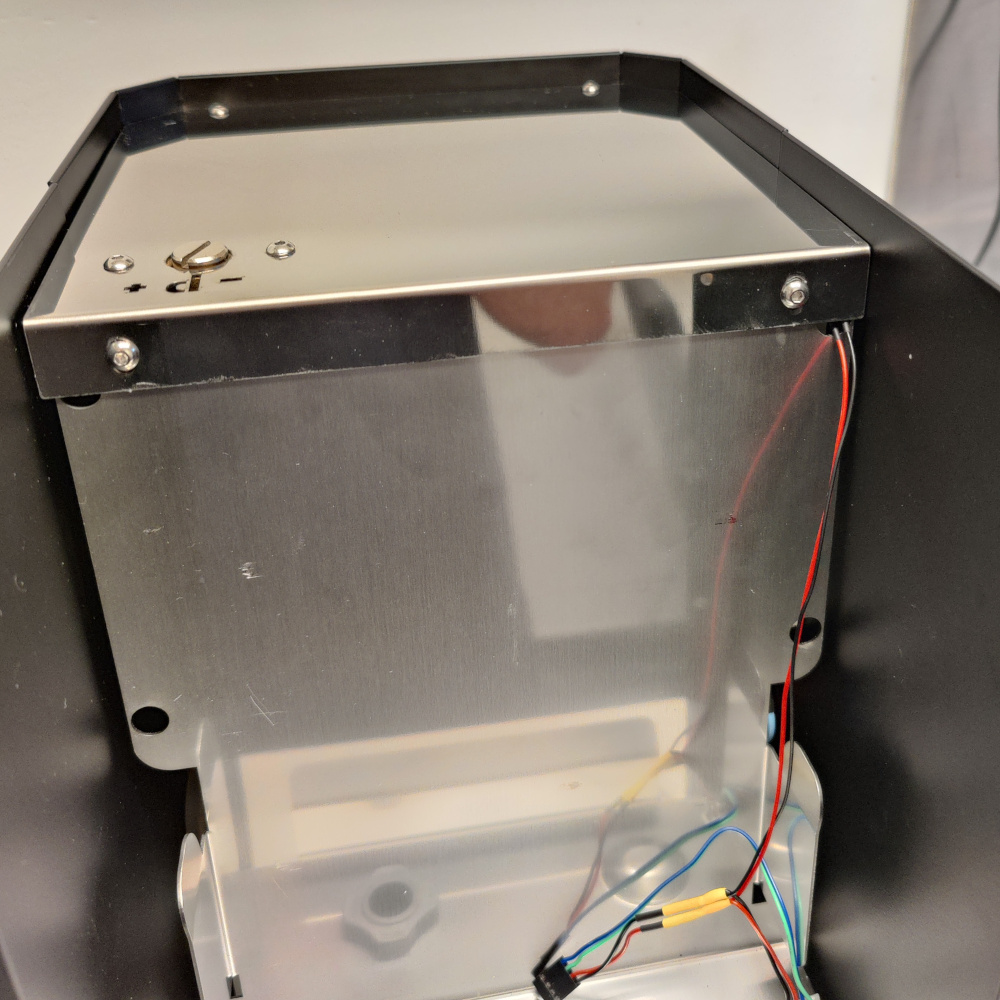
\includegraphics[width=\linewidth]{images/03_installation/17_close_top.jpg}
\end{minipage}

\subsubsection{Connection check}
\begin{minipage}[t]{0.5\linewidth}
	\vspace{0pt}
	Connect The 4-Pin Dupont of the wire harness and the two 2-Pin Duponts from the display cable as shown in the first image. Again, the TX of the display has to be connected to the RX of the level sensor and vice-versa. Your color coding might be different. If not done already, connect the display unit to the display cable outside of the machine. Place the water-tank lid with the level sensor on the topplate, with the sensor facing the topplate. Connect the level sensor to the wire harness. Plug in the machine. Verify that the display shows a 99 percent blue indicator. If the indicator is still orange with a question mark, the display could not communicate with the level sensor. In that case, doublecheck the RX-TX connection and all other plugs. If everything works, unplug the machine again and unplug the levelsensor.
\end{minipage}
\hfill
\begin{minipage}[t]{0.4\linewidth}
	\vspace{0pt}
	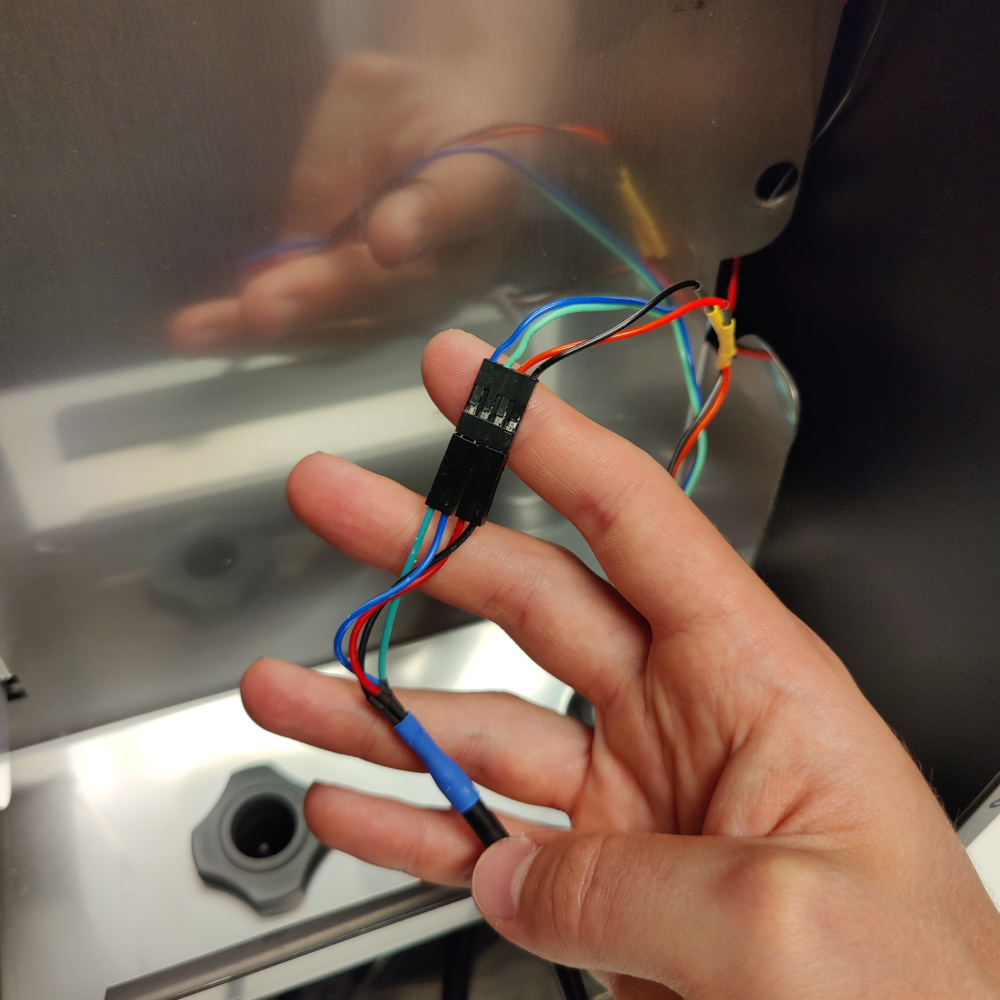
\includegraphics[width=\linewidth]{images/03_installation/18_connect_display.jpg}
	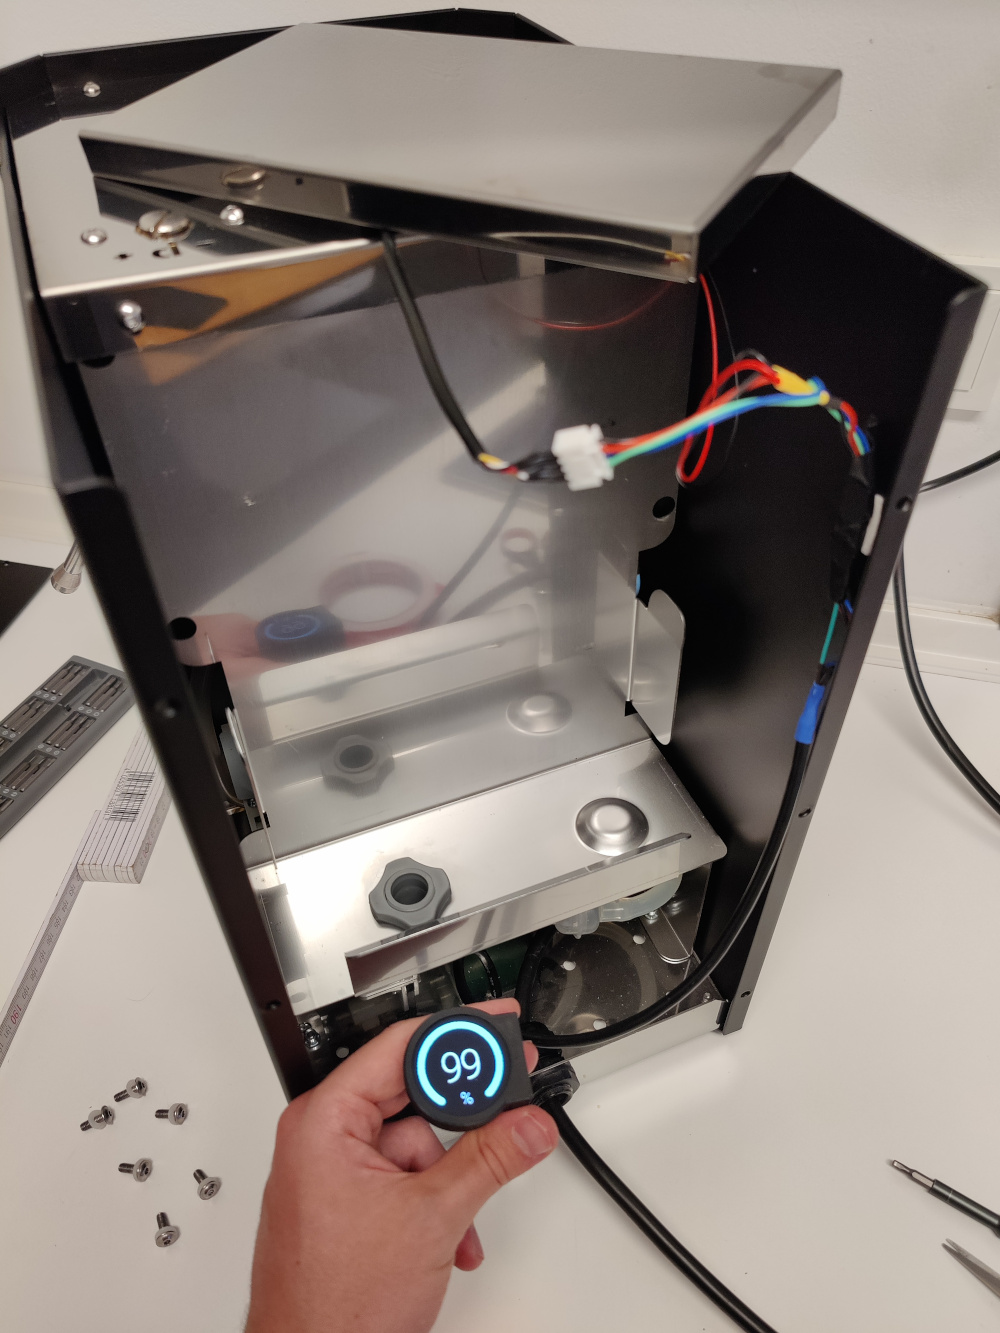
\includegraphics[width=\linewidth]{images/03_installation/19_function_check.jpg}
\end{minipage}

\subsubsection{Cable management and backplate}
\begin{minipage}[t]{0.5\linewidth}
	\vspace{0pt}
	I recommend wrapping some isolation tape around the Dupont connectors and sticking the to the upper edge of the machine with double-sided tape as shown in the picture. Make sure you are able to pull the 4-Pin JST-XH connector of the wire harness for the level-sensor higher out of the machine (this will make it easier to remove the level sensor when the machine is assembled). Afterwards, reinstall the backplate by performing the steps of section \ref{sec:backplate} in reverse. Be careful not to damage any cables.
\end{minipage}
\hfill
\begin{minipage}[t]{0.4\linewidth}
	\vspace{0pt}
	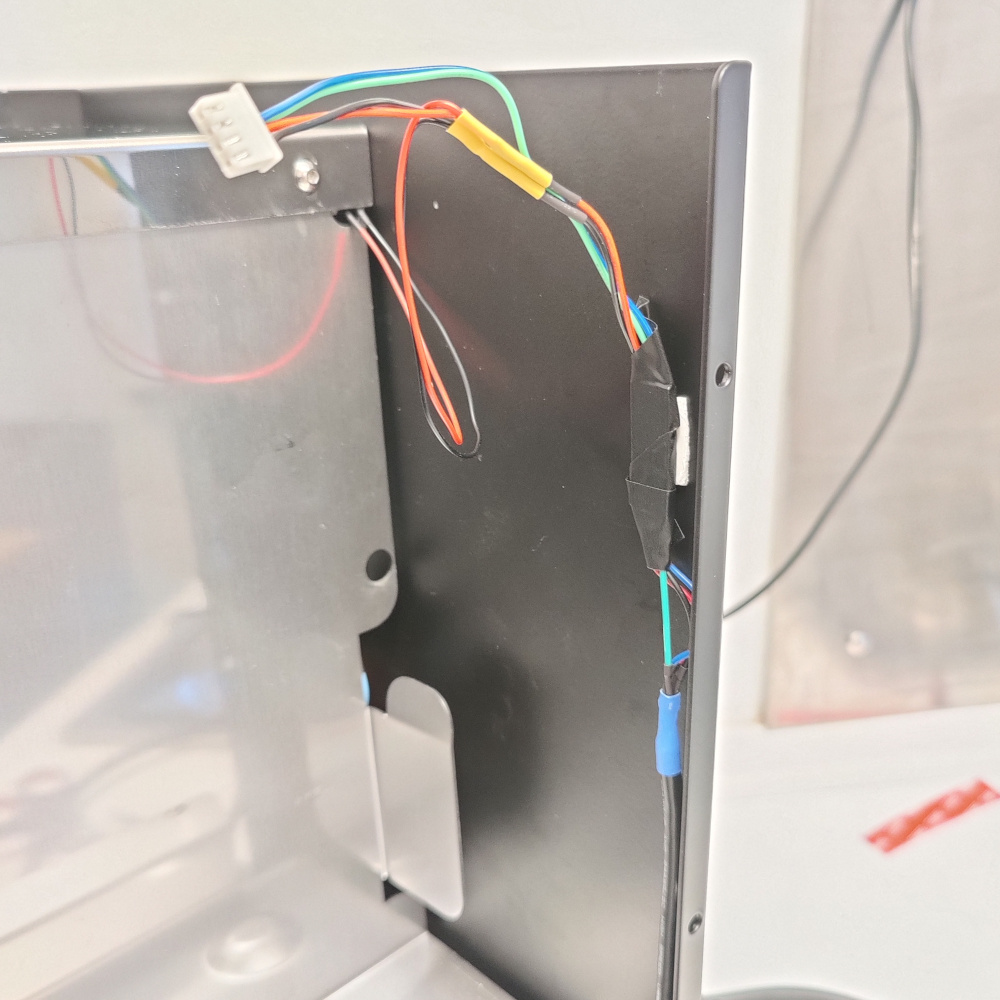
\includegraphics[width=\linewidth]{images/03_installation/20_attach_cables_to_machine.jpg}
\end{minipage}

\subsubsection{Finishline}
\begin{minipage}[t]{0.5\linewidth}
	\vspace{0pt}
	Reinstall the water-tank. Pull the 4-Pin JST-XH connector out of the machine while doing so (first picture). Make sure the water-tank doesn't sit on any other cables. Reconnect the level sensor (second picture). Push the JST-XH connector plug and any excess sensor cables under the ledge of the water-tank to hide them (third picture). The lid should close as normal, without any cable visible. That's it. You have successfully installed the mod! Congratulations!
\end{minipage}
\hfill
\begin{minipage}[t]{0.4\linewidth}
	\vspace{0pt}
	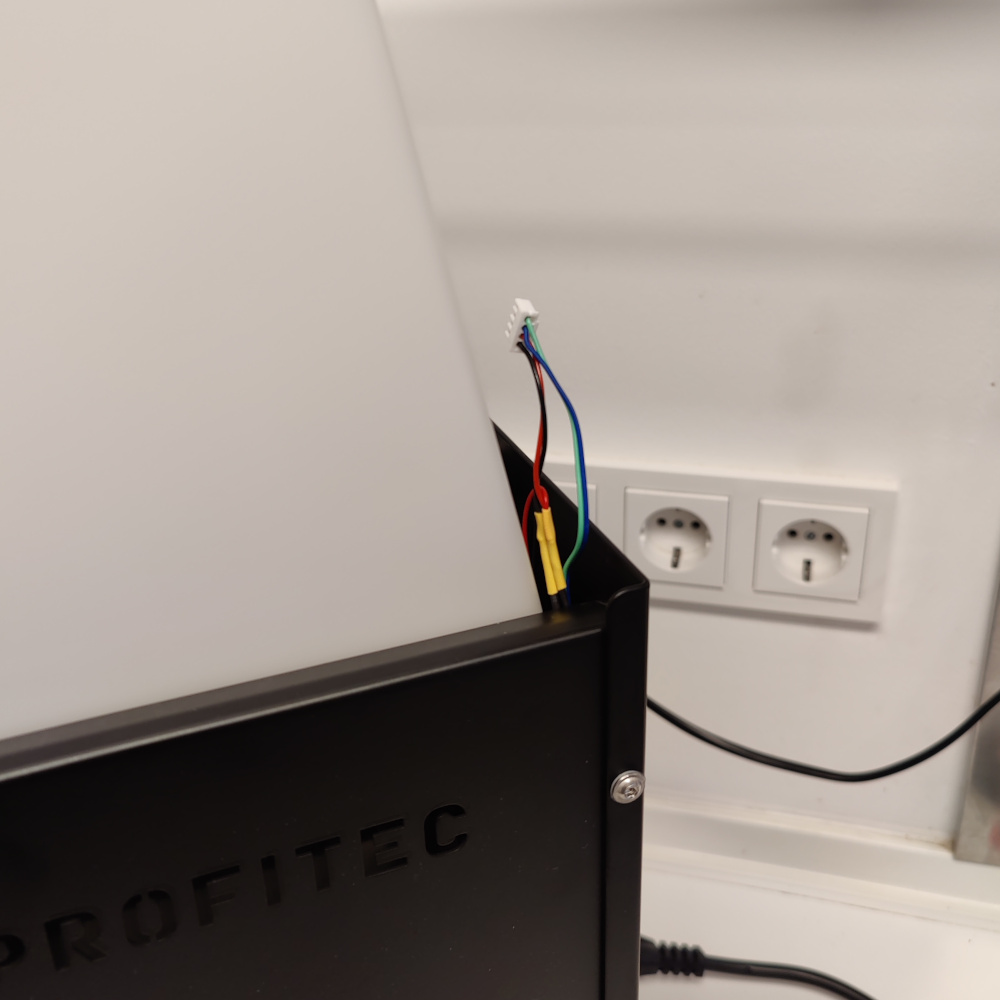
\includegraphics[width=\linewidth]{images/03_installation/21_reinstall_back_watertank.jpg}
	\includegraphics[width=\linewidth]{images/03_installation/22_connect_sensor.jpg}
	\includegraphics[width=\linewidth]{images/03_installation/23_hide_plug_refill_close_lid.jpg}
\end{minipage}

\end{document}
